\documentclass[11pt, aspectratio=169]{beamer}

\usetheme{metropolis}
\usepackage{appendixnumberbeamer}

\usepackage{booktabs}
\usepackage[scale=2]{ccicons}

\usepackage{pgfplots}
\usepgfplotslibrary{dateplot}

\usepackage{xspace}
\newcommand{\themename}{\textbf{\textsc{metropolis}}\xspace}

\usepackage[brazilian,hyperpageref]{backref}	 % Paginas com as citações na bibl
\usepackage[alf]{abntex2cite}	% Citações padrão ABNT

%Tabelas
\usepackage{tabularx}
\usepackage{adjustbox}
\usepackage{pgfplotstable}


% Equações
\newcommand{\dmc}{\(DMC_x^2\) }
\newcommand{\pdcca}{\({\rho}_{DCCA}\) }
\newcommand{\fdfa}{\(F_{DFA}\) }


% \newcommand{\dmc}{\(DMC_x^2\) }

% \usepackage{xparse} % for NewDocumentCommand
% \DeclareRobustCommand{\pdcca}{\raisebox{1.2\depth}{$\boldsymbol{\rho}$}$_{DCCA}$}
% \newcommand{\pdcca}{\raisebox{1.2\depth}{$\boldsymbol{\rho}$}$_{DCCA}$}
% \newcommand{\pdcca}{\scalebox{1.2}[1.0]{\ensuremath{\gamma}}}
\newcommand{\dfa}{$DFA$}
\newcommand{\dcca}{$DCCA$}

% \newcommand{\fdfa}{$F_{DFA}$}

% Dados da apresentação

\title{\pdcca~e \dmc~: Implementação, Otimização e Aplicações}
\subtitle{Defesa de Tese}
%\date{\today}
\date{23/05/2024}
\author{Discente: Fernando Ferraz Ribeiro \\Orientador: Prof. Dr.Gilney Figueira Zebende \\Coorientador: Prof. Dr. Juan Alberto Leyva Cruz}

\institute{PPGM UEFS - Feira de Santana, BA}

\titlegraphic{\hfill
\includegraphics[height=1.0cm]{../Figures/Logo_Uefs.jpg}
\includegraphics[height=1.0cm]{../Figures/logoPPGM-UEFS.png}}

\begin{document}

\maketitle

\begin{frame}{Sumário}
  \setbeamertemplate{section in toc}[sections numbered]
  \tableofcontents[hideallsubsections]
\end{frame}

\section{Introdução}

\begin{frame}[fragile]{Sistemas Complexos}

  Este conjunto amplo de fenômenos é comumente identificado e agrupado por algumas de suas características: são formados pela contribuição de um conjunto (geralmente grande) de componentes (muitas vezes simples) que, interagindo, estruturam-se de forma auto-organizada, gerando resultados inesperados, que não podem ser previstos pelos estudos estatísticos e/ou matemáticos tradicionais dos elementos formadores do sistema.

\end{frame}

\begin{frame}
  \frametitle{Reconhecimento}

  Em 2021, a Academia Real das Ciências da Suécia concedeu metade do Prêmio Nobel de Física para Syukuro Manabe e Klaus Hasselmann, cujos estudos apresentam modelos complexos para a análise do clima. Em particular apontam uma correlação entre as emissões de dióxido de carbono e as mudanças climáticas.

\end{frame}

\begin{frame}
  \frametitle{Sistemas Complexos e Ciência de Dados}

  Muitos fenômenos complexos são investigados pela análise de grandes conjuntos de dados. É notável a velocidade e quantidade de dados que são gerados e armazenados pela humanidade atualmente. A aquisição, manipulação, gestão, armazenamento e criação de valor a partir de dados, através de ambientes computacionais, tem-se apresentado como um novo paradigma tecnológico. ...

\end{frame}

\begin{frame}
  \frametitle{Sistemas Complexos e Ciência de Dados}
  Um campo do conhecimento que recebeu a denominação de \textbf{Ciência de Dados}, conceito que envelopa alguns termos frequentemente associados à inovação científica, técnica e social como \textbf{Big Data, mineração de dados, Business Intelligence internet das coisas, inteligência artificial} e \textbf{aprendizado de máquina(AM)}, dentre outros \cite[p. 12-13]{EMCdata2015}.
\end{frame}

\begin{frame}
  \frametitle{Séries Temporais}

  As séries temporais são definidas como um conjunto de observações (numéricas ou categóricas) ordenado no tempo.  Embora muitos dos dados que descrevem as dinâmicas espaciais podem ser registrados na forma de sérias temporais (abastecimento de água nas tubulações, consumo de energia elétrica nos imóveis, fluxos de pessoas e veículos pela cidade, casos de uma doença por dia, etc.), contudo as técnicas de medição de correlações, bem como a devida exploração destas para inferir novos conhecimentos, permanecem como perguntas abertas em muitas sub-áreas das ciências ambientais\cite{Bermudez-Edo2018}.

\end{frame}

\begin{frame}{Definição do Problema}

  O coeficiente \dmc~é uma ferramenta promissora para a análise de correlações em séries temporais múltiplas. No entanto, sua aplicação ainda é limitada devido à falta de implementações computacionais eficientes e estudos que explorem seu potencial em diferentes contextos.


\end{frame}

\begin{frame}{Objetivo Principal}

  Investigar a aplicabilidade do \pdcca~e do \dmc com o objetivo, não só de identificar correlações entre variáveis, mas também de entender o algoritmo, propor e aperfeiçoar ferramentas computacionais para a realização dos cálculos.


\end{frame}

\begin{frame}{Objetivos Gerais}

\begin{enumerate}
    \label{enum:obj_espec}
    \item  Testar os algoritmos e os métodos.
    \item Implementar um algoritmo computacional geral para calcular o \dmc para qualquer número de séries temporais.
    \item Testar as ferramentas implementadas em novas análises.
\end{enumerate}

\end{frame}

\begin{frame}
  \frametitle{Premissas}

\begin{enumerate}
  \label{enum:premissas}

  \item O \dmc, pelas características de análise do método, pode ajudar a entender características de séries temporais e aplicado em problemas de diversas áreas.
  \item O \dmc~é uma generalização do método \pdcca~para múltiplas séries temporais.
	\item O \pdcca, em determinadas condições testadas, apresentou resultados mais interessantes (como melhor descrição dos fenômenos) que os apresentados pelo coeficiente de Pearson quando aplicado à séries temporais não estacionárias~\cite{Wang2013}. 
\end{enumerate}

\end{frame}

\begin{frame}
  \frametitle{Hipóteses}

\begin{enumerate}
    \item É possível otimizar os cálculos do \pdcca~e do \dmc.
    \item Com maior poder de cálculo a aplicação dos coeficientes seria potencializada.
	\item Uma ferramenta adequada para o cálculo dos coeficientes seria um impulso na utilização e divulgação destes.
\end{enumerate}

\end{frame}


\section{Metodologia}

\begin{frame}
\frametitle{Etapas do processo}
Abordagem experimental.

Etapas:
\begin{itemize}
  \item Revisão bibliográfica.
  \item Análise das ferramentas computacionais existentes.
  \item Proposta de uma nova ferramenta computacional.
  \item Implementação.
  \item Testes.
  \item Exploração das novas possibilidades de análise.
\end{itemize}

\end{frame}


\section{Fundamentação Teórica}


\begin{frame}[allowframebreaks]
\frametitle{DFA - \cite{Peng_1994}}
\begin{enumerate}
\item \textbf{Cálculo da série integrada}: dada uma série temporal $\{x_{i}\}$, com $i$ variando de $1$ a $N$, a série integrada $X_{k}$ é calculada por $X_{k} = \sum_{i=1}^{k}\left[x_{i} - \langle x \rangle \right]$, com $k$ também variando de $1$ a $N$;
\item \textbf{Divisão da série em caixa}s: a série integrada$X_{k}$ é dividida em $(N - n)$ caixas de tamanho $n$ (escala temporal), cada caixa contendo $n + 1$ valores, começando em $i$ até $i + n$;
\item \textbf{Cálculo do ajuste polinomial}: para cada caixa, é calculado polinômio (geralmente de grau 1) que melhor se ajusta, obtendo $\widetilde{X}_{k, i}$ com $i \le k \le (i + n)$;
\item \textbf{Cálculo da função $f_{DFA}^{2}$ para cada caixa}: para cada caixa de uma escala temporal é calculada a função de \dfa~pela expressão:\\[10pt]
 $f_{DFA}^{2}(n, i) = \frac{1}{1+n} \sum_{k=i}^{i + n}(X_{k,i}-\widetilde{X}_{k,i})^{2}$;
\item \textbf{Cálculo da função de flutuação para uma escala temporal}: para todas as caixas de uma escala de tempo, o DFA é calculado como: \\[10pt]
        $F_{DFA}(n) = \sqrt{\frac{1}{N - n} \sum_{i=1}^{N-n} f_{DFA}^{2}(n, i)}$;
\item \textbf{Análise em diferentes escalas temporais}: para diferentes escalas de tempo ($n$), com valores possíveis $4 \le n \le \frac{N}{4}$, é calculada a função $F_{DFA}$ para encontrar uma relação entre $F_{DFA} \times n$
  \end{enumerate}

\end{frame}

\begin{frame}[allowframebreaks]
\frametitle{DCCA - \cite{Podobnik2008}}
\begin{enumerate}
    \item \textbf{Cálculo das séries integradas}: tomando duas séries temporais com a mesma extensão $\{x^{j1}_{i}\}$ e $\{x^{j2}_{i}\}$ com $i$ variando de $1$ a $N$,
          as séries integradas $X\alpha_{k}$ e $X\beta_{k}$ são calculadas por
          $X_{k} = \sum_{i=1}^{k}\left[x_{i} - \langle x \rangle \right] $ para cada série, com $k$ também variando de $i$ a $N$;
    \item \textbf{Divisão das séries em caixas}: as séries $X^{j1}_{k}$ e $X^{j2}_{k}$ são divididas em $(N - n)$ caixas de tamanho $n$ (escala de tempo), cada caixa contendo $n + 1$ valores, começando em $i$ até $i + n$;
    \item \textbf{Cálculo dos ajustes de polinômios}: para cada caixa, um polinômio (geralmente de grau 1) melhor se ajusta, obtendo
          $\widetilde{X^{j1}}_{k, i}$ e $\widetilde{X^{j2}}_{k, i}$,
          para séries $\{x^{j1}_{i}\}$ e $\{x^{j2}_{i}\}$ respectivamente,
          com $i \le k \le (i + n)$;
    \item \textbf{Cálculo da função $f_{DCCA}^{2}$~em cada caixa}: para cada caixa uma das $N - n$ caixas de uma mesma escala temporal a função é calculada por:\\[10pt]
     $f_{DCCA}^{2}(n, i) =
            \frac{1}{1+n} \sum_{k=i}^{i + n}(X^{j1}_{k,i}-\widetilde{X^{j1}}_{k, i}) \times (X^{j2}_{k,i}-\widetilde{X^{j2}}_{k, i})$
    \item \textbf{Cálculo do \dcca~para toda a escala temporal}: para todas as caixas de uma mesma escala temporal, o \dcca~é calculado como:\\[10pt]
          $F_{DCCA}(n) = \sqrt{\frac{1}{N - n} \sum_{i=1}^{N-n} f_{DCCA}^{2}(n, i)}$;
    \item \textbf{Análise em diferentes escalas temporais}: para um número de escalas de tempo ($n$), com valores possíveis $4 \le n \le \frac{N}{4}$, o \dcca~é calculado para encontrar uma relação entre $F_{DCCA} \times n$

\end{enumerate}

\end{frame}

\begin{frame}
\frametitle{\pdcca - \cite{Zebende2011}}

\begin{equation}
  {\rho}_{DCCA}(n) = \frac{F_{DCCA~(x^{j1},~x^{j2})}^{2}(n)}
  {F_{DFA~(x^{j1})}(n) \times F_{DFA~(x^{j2})}(n)}
  \label{eq:p_dcca}
\end{equation}

\end{frame}

\begin{frame}
  \frametitle{\dmc - \cite{Zebende2018}}

  \begin{equation}
  {DMC}_{x}^{2}  \equiv \rho_{Y,X^{j}}(n)^{T} ~\times ~ \rho^{-1}(n) ~\times ~\rho_{Y,X^{j}}(n)
  \label{eq:dmc}
\end{equation}

\begin{equation} \label{eq:rho_vec_col}
  \rho_{Y,X^{j}}(n)^T=[\rho_{Y,X^1}(n), \rho_{Y,X^2}(n),\cdots,\rho_{Y,X^m}(n)]
\end{equation}

\begin{equation}
  \rho~(n) = \left(\begin{matrix}
    1                     & \rho_{X^{1},X^{2}}(n) & \rho_{X^{1},X^{3}}(n) & \dots & \rho_{X^{1},X^{m}}(n) \\
    \rho_{X^{2},X^{1}}(n) & 1                     & \rho_{X^{2},X^{3}}(n) & \dots & \rho_{X_{2},X^{m}}(n) \\
    \vdots                & \vdots                & \vdots                & \dots & \vdots                \\
    \rho_{X^{m},X^{1}}(n) & \rho_{X^{m},X^{2}}(n) & \rho_{X^{m},X^{3}}(n) & \dots & 1                     \\
  \end{matrix}\right)
  \label{eq:p_dcca_matrix}
\end{equation}

\end{frame}

\begin{frame}
  \frametitle{Variações do \dfa.}

   \begin{figure}[!htb]
    \centering
    \caption{Diagrama}
    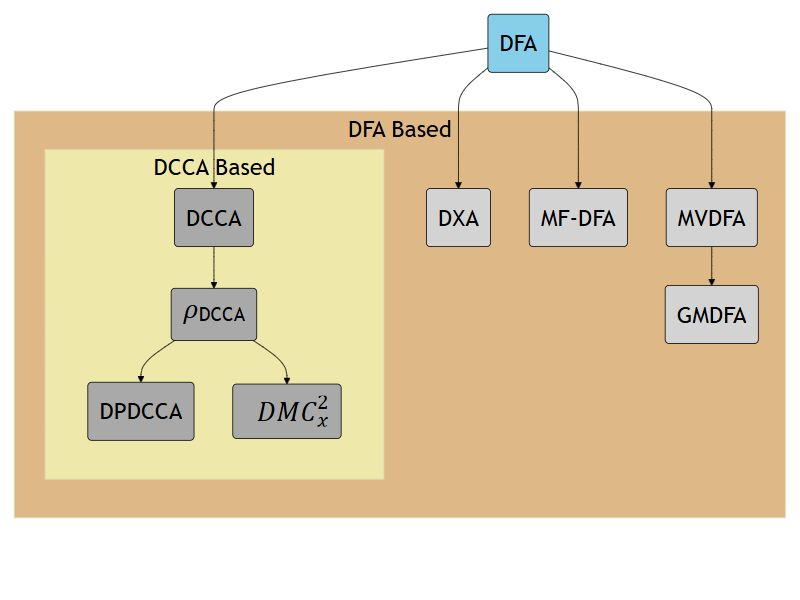
\includegraphics[height=.8\paperheight]{./diag_revisao.jpeg}
    \label{fig:diag_revisao}
  \end{figure}

\end{frame}

\section{Resultados}

\subsection{Artigo 01}

\begin{frame}
  \frametitle{Artigo 01 - Publicado}

  \begin{figure}[!htb]
    \centering
    \caption{\cite{Oliveira2023}}
    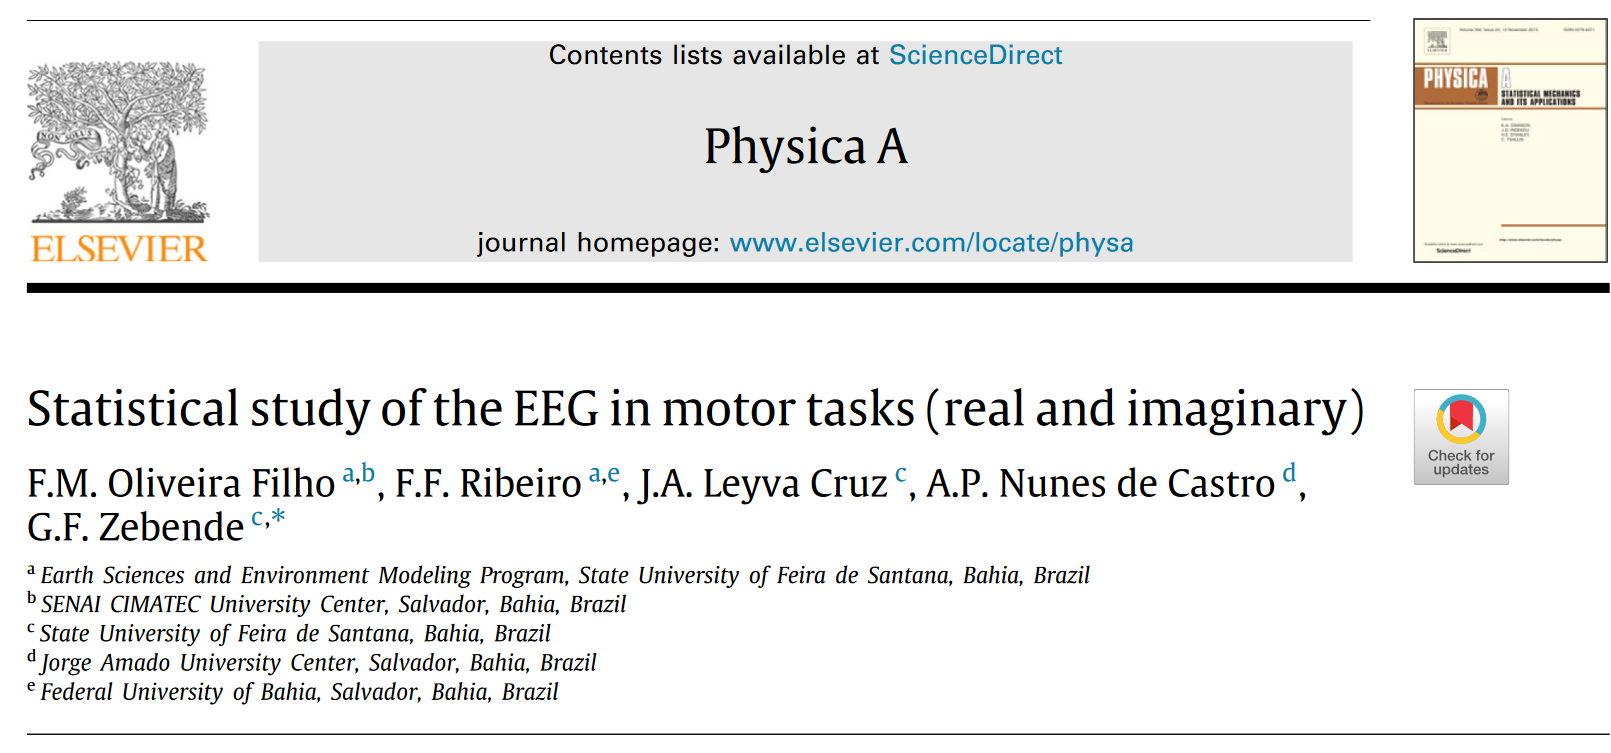
\includegraphics[height=.6\paperheight]{../Figures/artigos_publicados/artigo_01_abr_2023.png}
    \label{fig:ar_pub_01}
  \end{figure}

\end{frame}

% \section{Considerações Finais}

% \begin{frame}{Considerações Finais}
\begin{frame}
  \frametitle{Algoritmo registrado}

  \begin{figure}[!htb]
    \centering
    \caption{Registro de Software}
    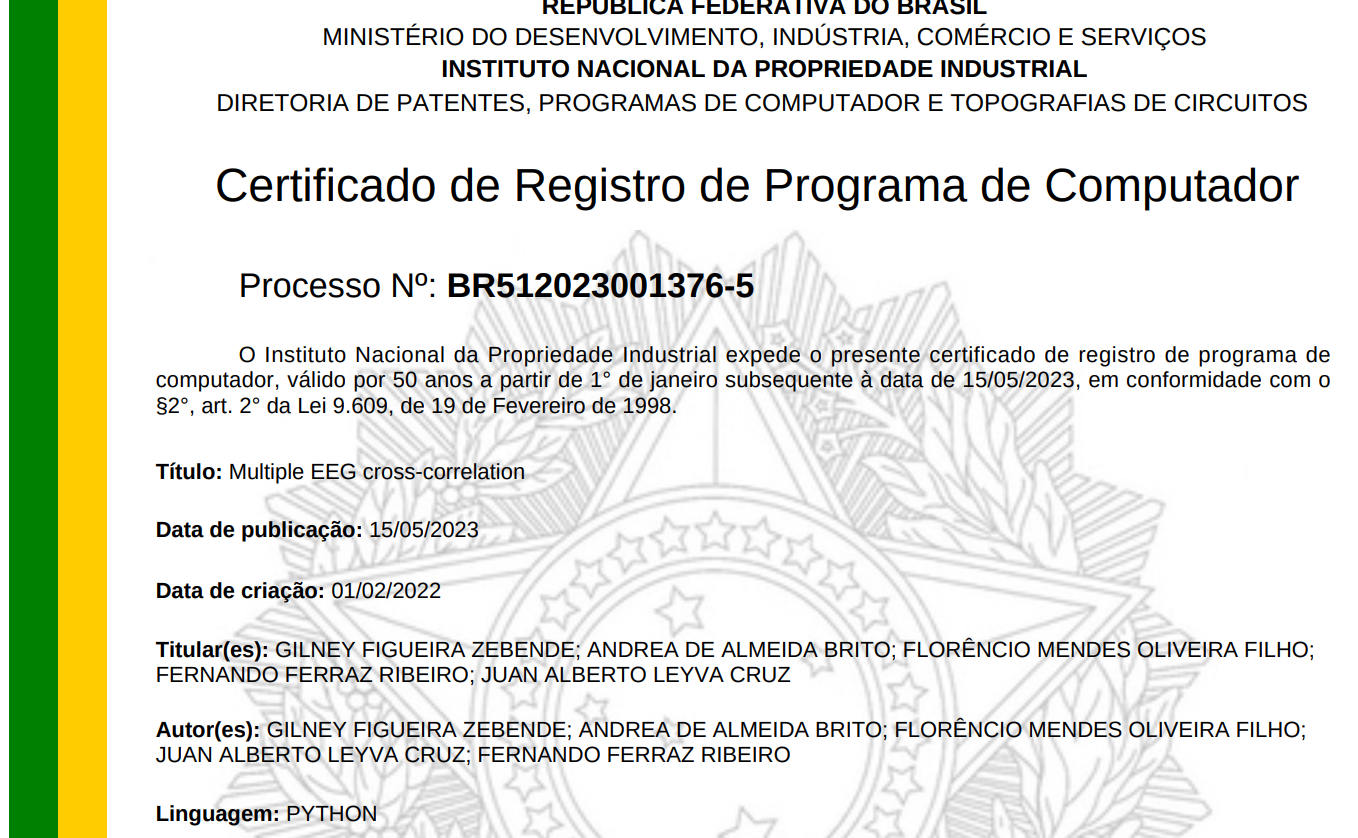
\includegraphics[height=.6\paperheight]{../Figures/artigos_publicados/certificado_alg_01.png}
    \label{fig:alg_pub_01}
  \end{figure}

\end{frame}


\subsection{Algoritmo registrado - 01}

\begin{frame}
  \frametitle{Algoritmo registrado - 01}

  \begin{equation}
    \begin{split}
      DMC_{x}^{2} \quad = \quad & \Big( \Big. \rho^{2}_{X_{2},X_{3}} \times \rho^{2}_{Y,X_{1}}- \rho^{2}_{Y,X_{1}} + \rho^{2}_{X_{1},X_{3}}\times \rho^{2}_{Y,X_{2}}-\rho^{2}_{Y,X_{2}} \\
      &+ 2 \times \rho_{X_{1},X_{2}} \times \rho_{Y,X_{1}} \times \rho_{Y,X_{2}}   - 2 \times \rho_{X_{1},X_{3}} \times \rho_{X_{2},X_{3}} \times \rho_{Y,X_{1}} \\
      &+ \rho^{2}_{X_{1},X_{2}} \times \rho^{2}_{Y,X_{3}}-\rho^{2}_{Y,X_{3}} + 2 \times \rho_{X_{1},X_{3}} \times \rho_{Y,X_{1}} \times \rho_{Y,X_{3}} \\
      &- 2 \times \rho_{X_{1},X_{2}} \times \rho_{X_{2},X_{3}} \times \rho_{Y,X_{1}} \times \rho_{Y,X_{3}} \\
      &- 2 \times \rho_{X_{1},X_{2}} \times \rho_{X_{1},X_{3}} \times \rho_{Y,X_{2}} \times \rho_{Y,X_{3}} \\
      &+ 2 \times \rho_{X_{2},X_{3}} \times \rho_{Y,X_{2}} \times \rho_{Y,X_{3}} \Big. \Big)    \quad \Big/ \\
      & \Big( \Big. \rho^{2}_{X_{1},X_{2}} + \rho^{2}_{X_{1},X_{3}} + \rho^{2}_{X_{2},X_{3}} - 2 \times \rho_{X_{1},X_{2}} \times \rho_{X_{1},X_{3}} \times \rho_{X_{2},X_{3}}^{-1}\Big. \Big)  \\
    \end{split}
    \label{eq:dmc_3x_y}
  \end{equation}

\end{frame}

\subsection{Artigo 02}

\begin{frame}
  \frametitle{Artigo 02}

  \textbf{\Large{Multi Cross-correlation Analysis in a Multi-channel EEG applied in Motor Activity (Real/Imaginary)}}
  \medskip
  \begin{center}
    \url{https://255ribeiro.github.io/Multi_Cross-correlation_EEG/}
  \end{center}
 

\end{frame}

\begin{frame}
  \frametitle{Artigo 02}
  \begin{figure}[!h]
    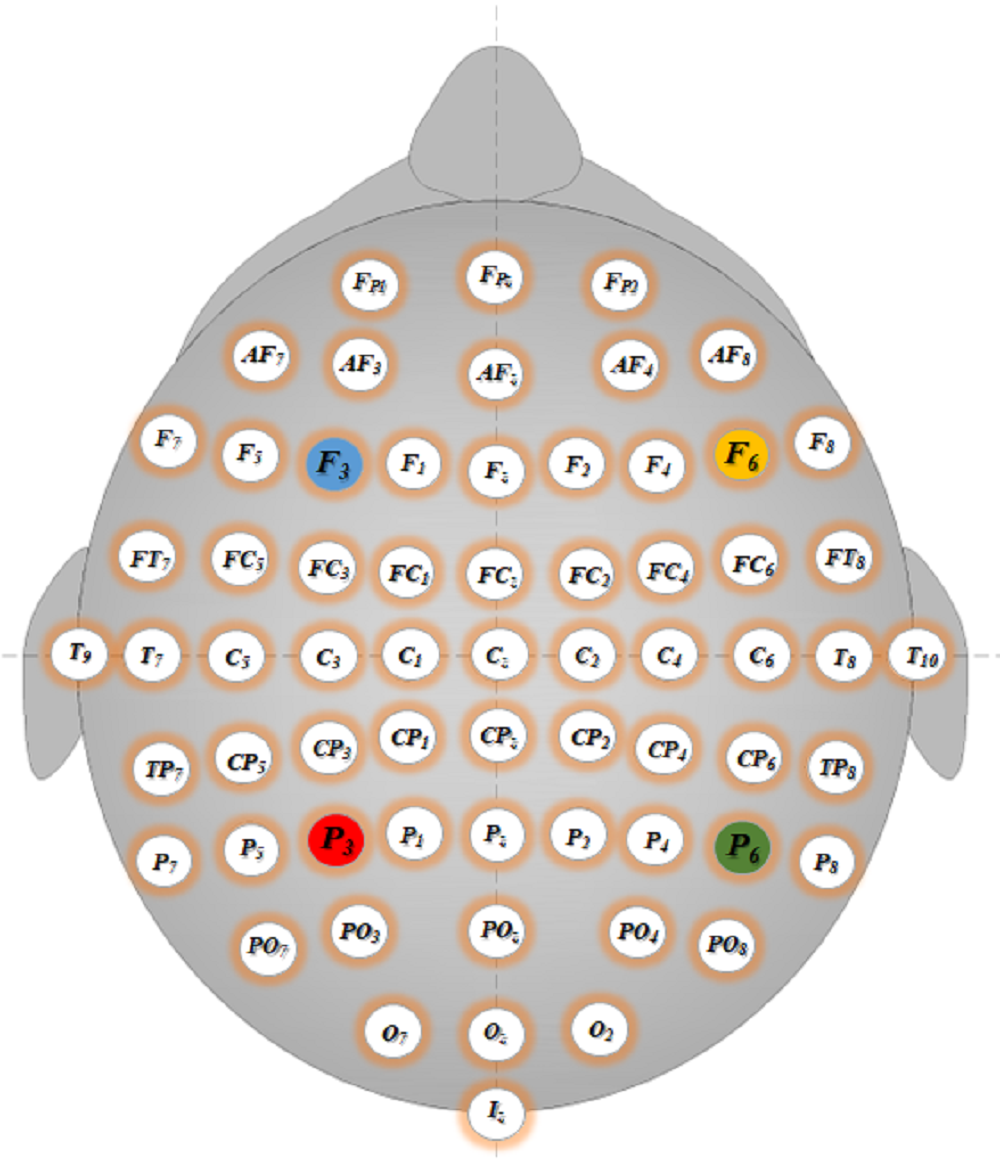
\includegraphics[height=.6\paperheight]{../Figures/art_02/Fig1.png}
    \caption{Posição dos canais de EEG e canais utilizados}
    \label{fig01}
  \end{figure}
\end{frame}



\begin{frame}
  \frametitle{Artigo 02}

  \begin{figure}[!h]
    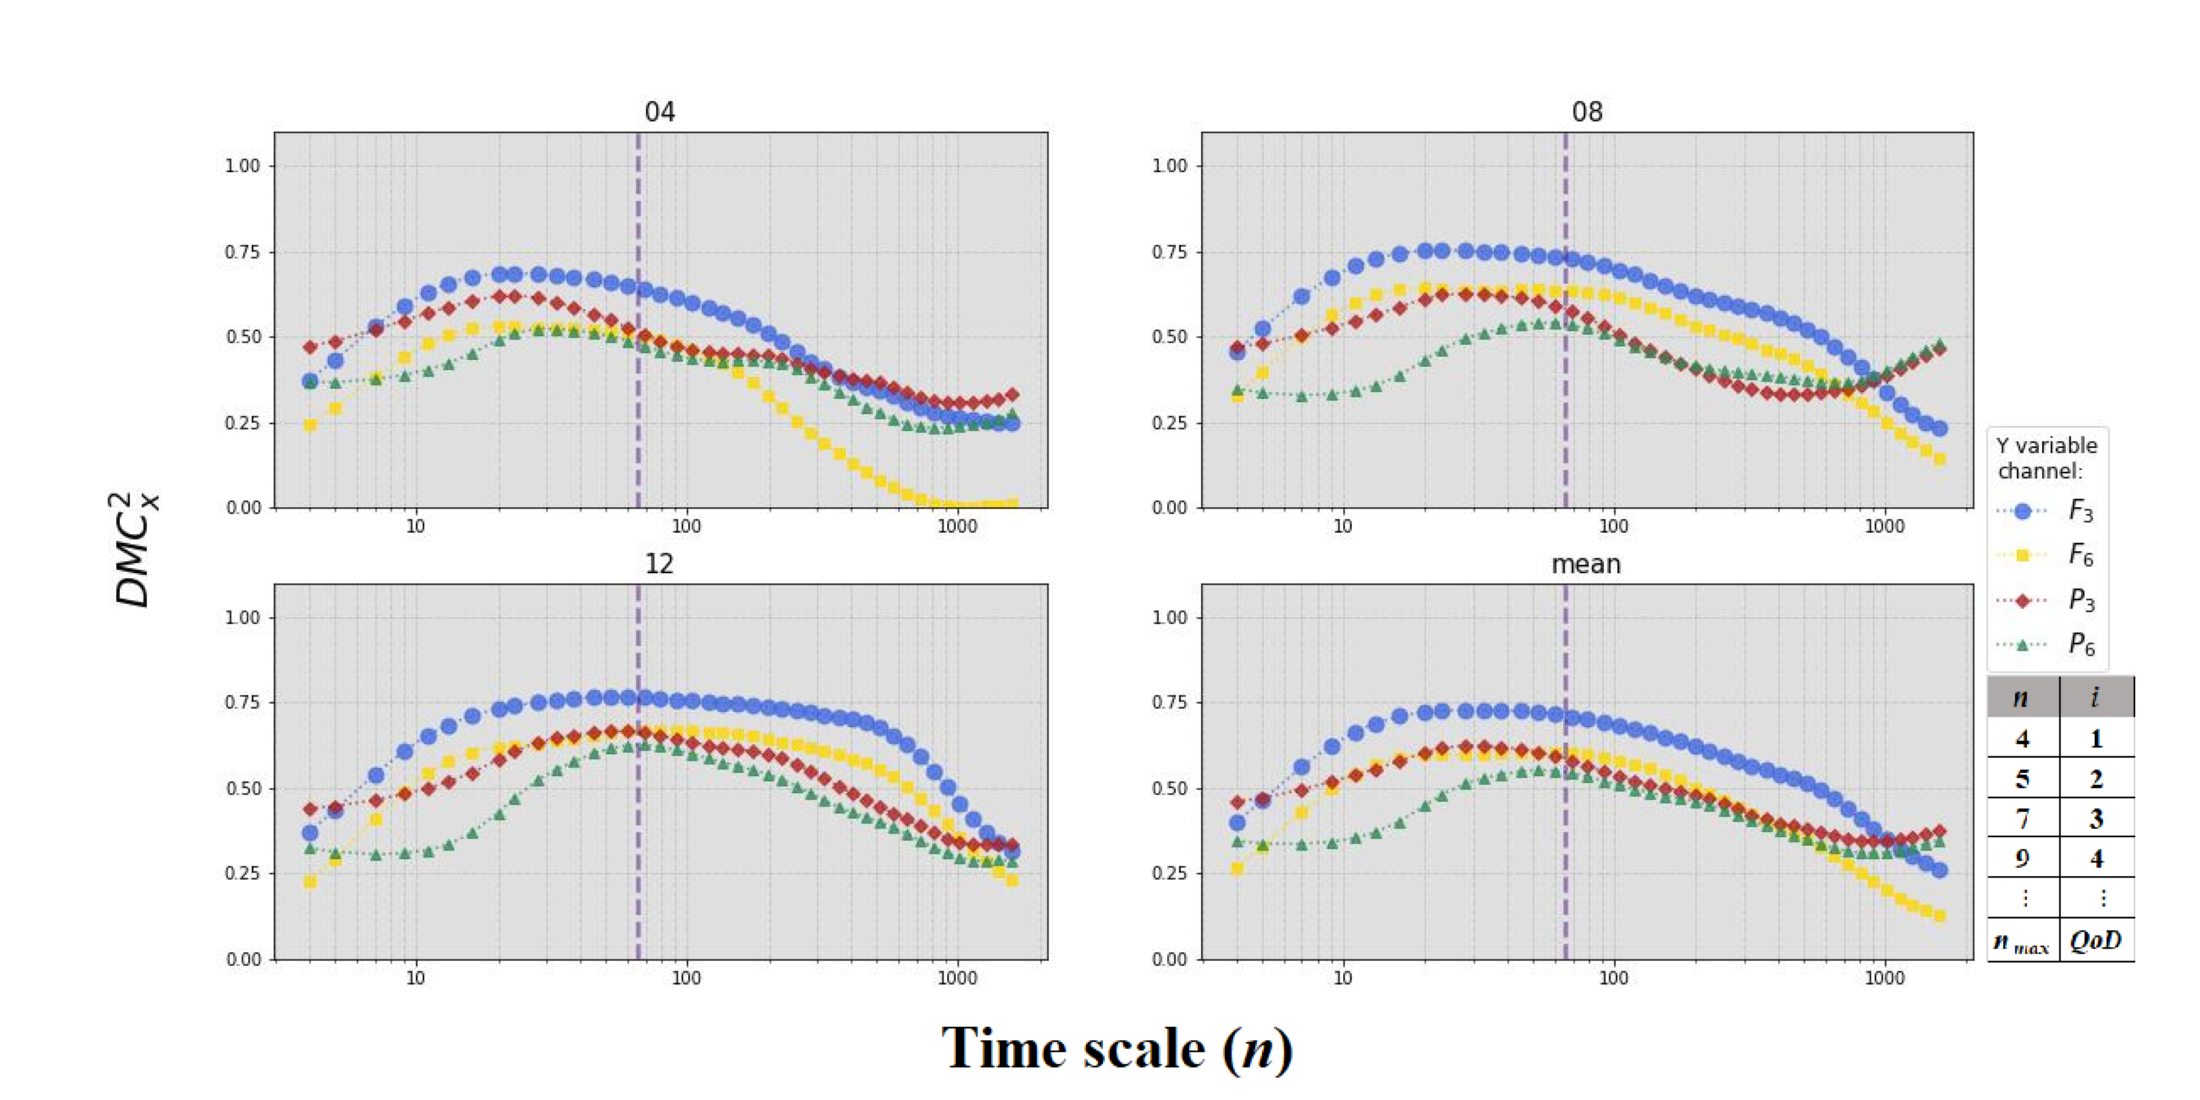
\includegraphics[height=.5\paperheight]{../Figures/art_02/Fig2.png}
    \caption{$DMC_{x}^{2}$ as a function of time scale $n$. Here is showing the results for subject S014 recordings for Task 2, presenting experiments 04, 08, 12 and the mean values for these experiments. The vertical line represents $n=67$ and $QoD$ is the total amount of time scales involved in $DMC_{x}^{2}$ calculations.}
    \label{fig02}
  \end{figure}
\end{frame}


\begin{frame}
  \frametitle{Artigo 02}

  %%%%%%%%%%%%%%%%%%%
  \begin{figure}[!h]
    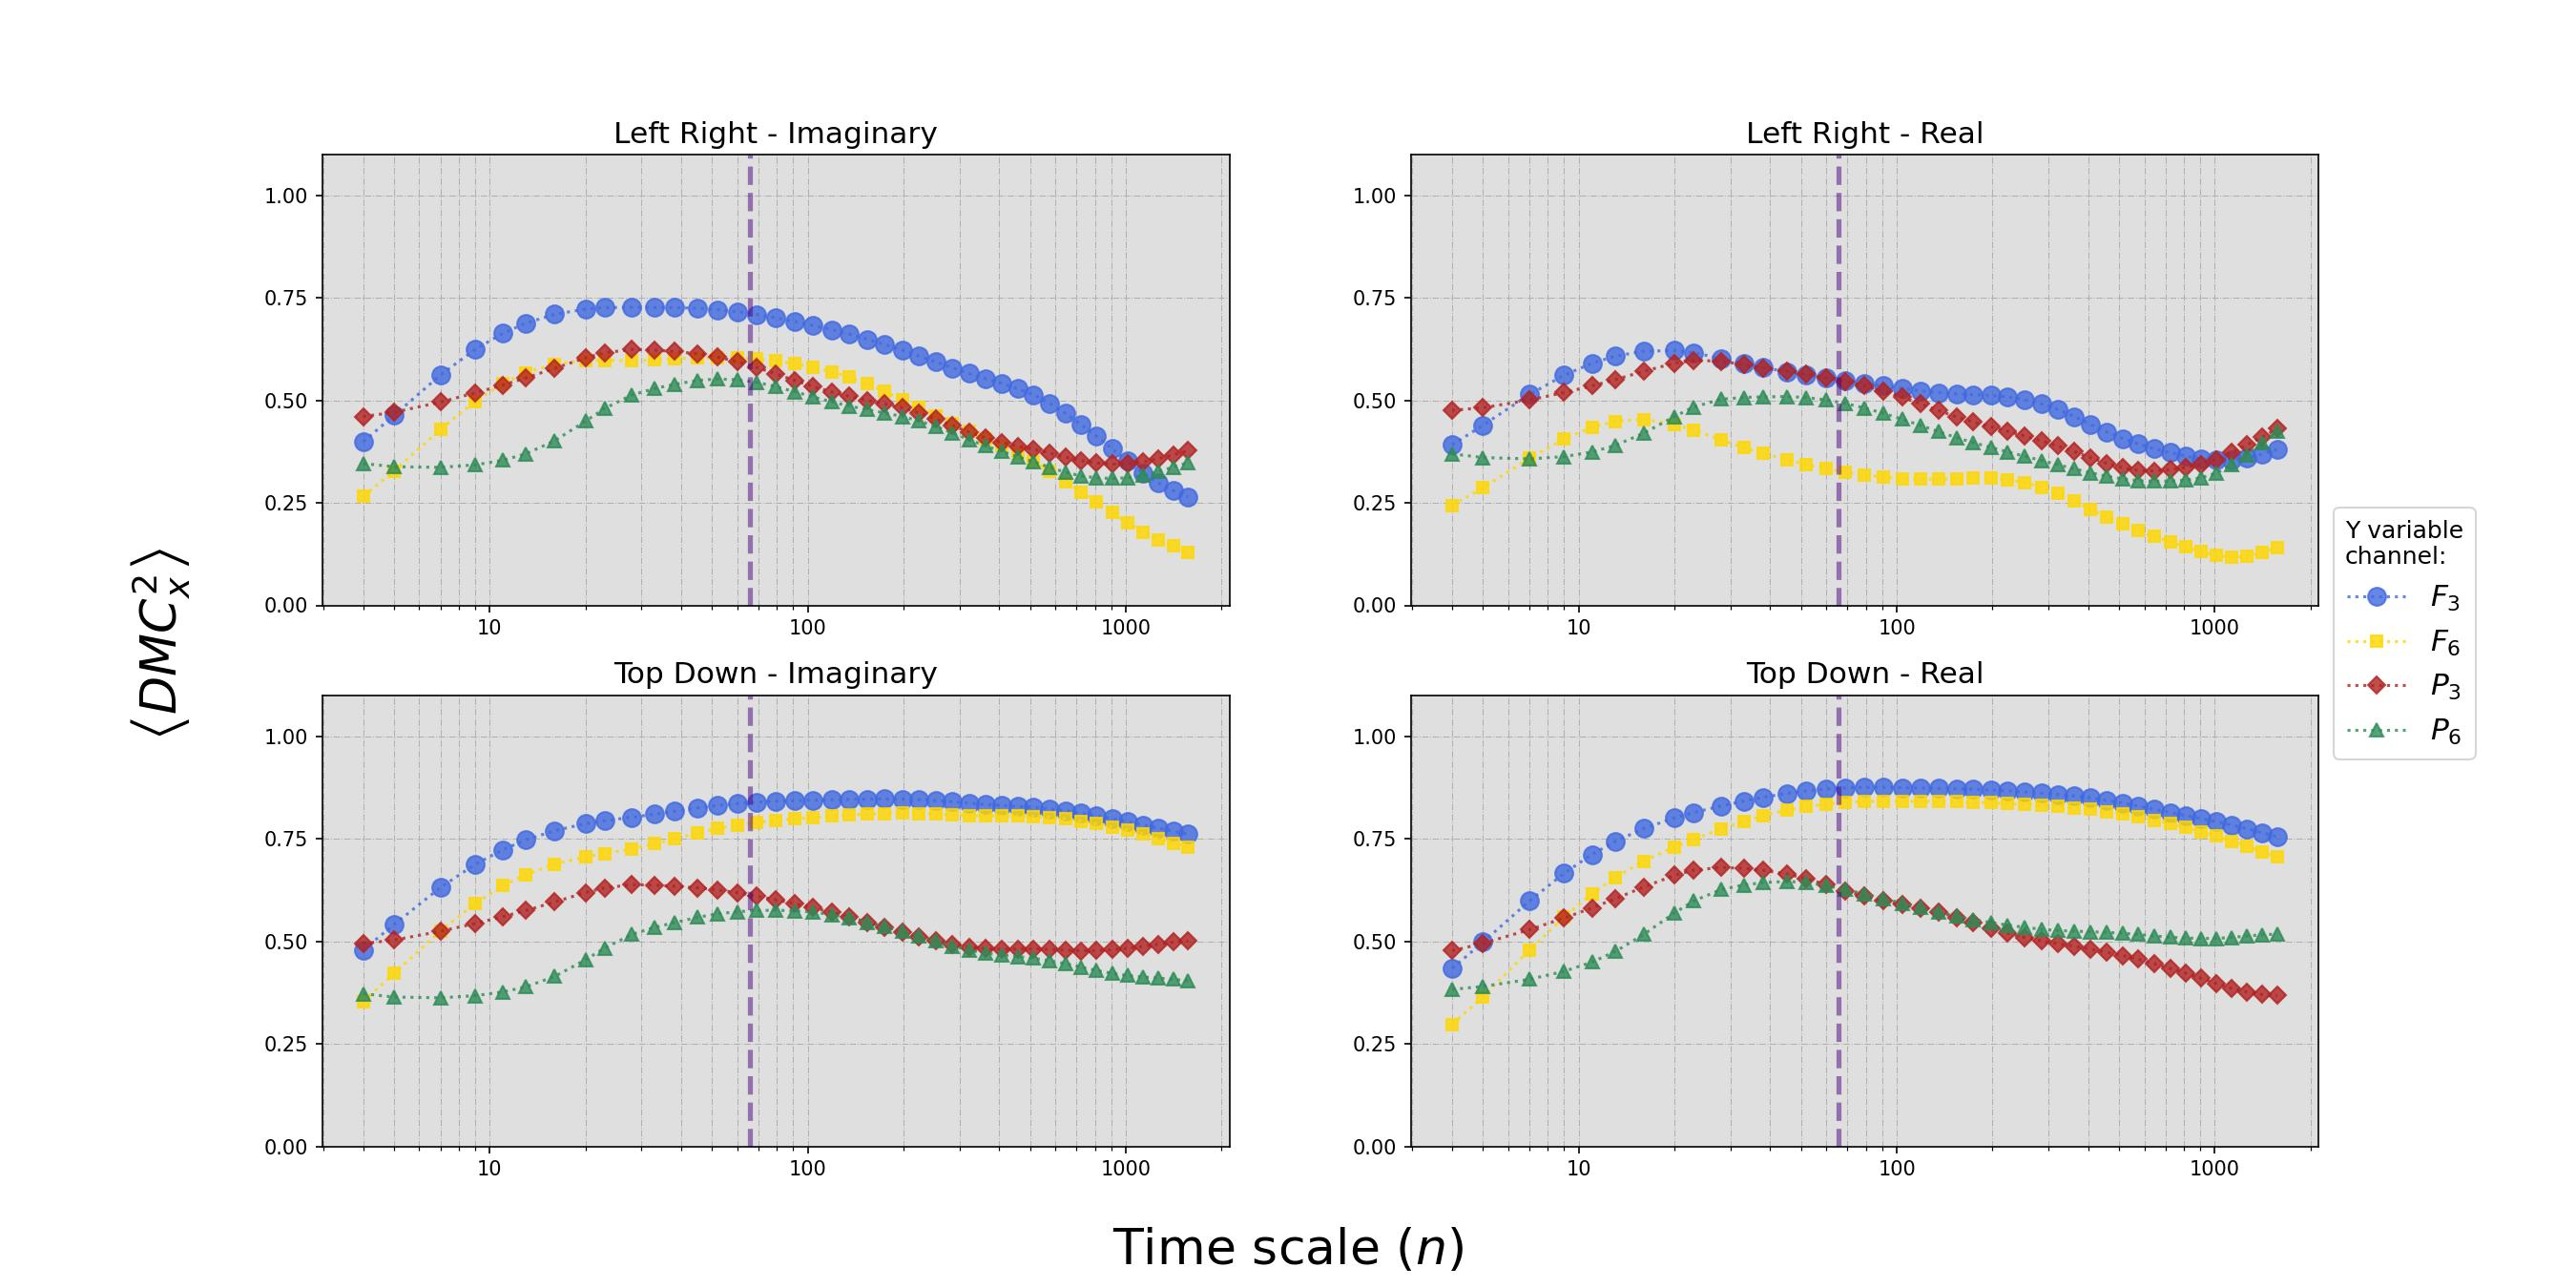
\includegraphics[height=.5\paperheight]{../Figures/art_02/Fig3.jpg}
    \caption{Mean values of $DMC_{x}^{2} \times n$ for all Tasks: Left/Right (Imaginary), Left/Right (Real), Top/Down (Imaginary), and Top/Down (Real) for the S014 subject.}
    \label{fig03}
  \end{figure}
  %%%%%%%%%%%%%%%%%%%
\end{frame}


\begin{frame}
  \frametitle{Artigo 02}

  %%%%%%%%%%%%%%%%%%%
  \begin{figure}[!h]
    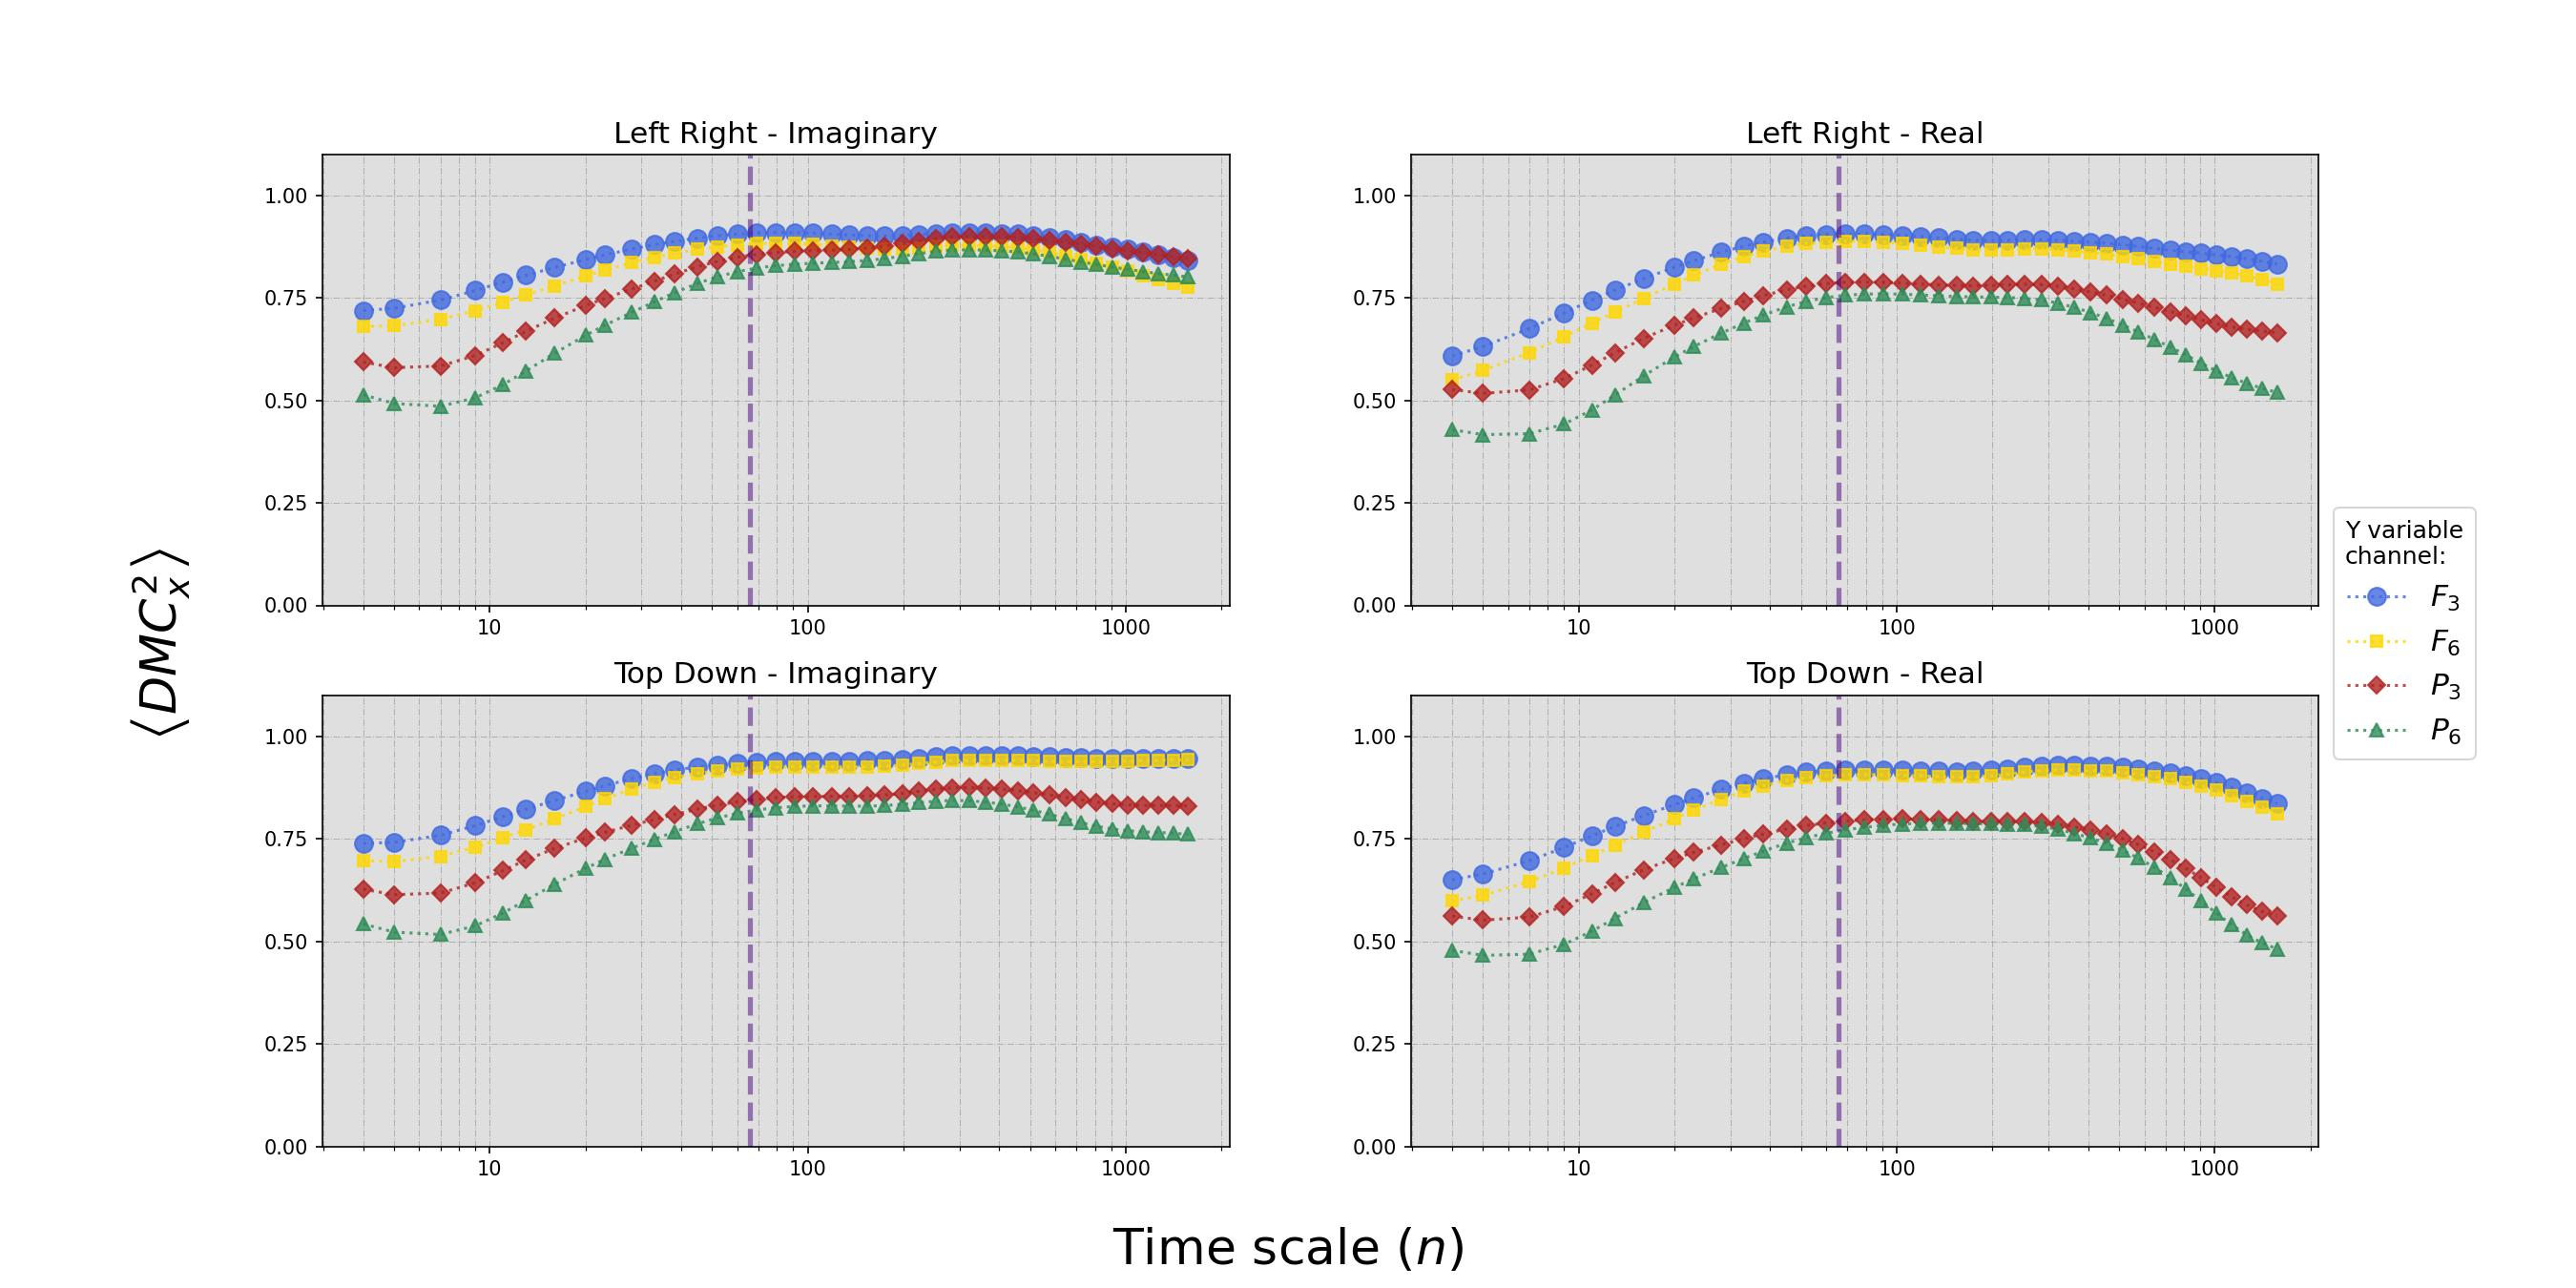
\includegraphics[height=.5\paperheight]{../Figures/art_02/Fig4.jpg}
    \caption{Mean values of $DMC_{x}^{2} \times n$ for all Tasks: Left/Right (Imaginary), Left/Right (Real), Top/Down (Imaginary), and Top/Down (Real) for the S036 subject.}
    \label{fig04}
  \end{figure}
  %%%%%%%%%%%%%%%%%%%
\end{frame}

\begin{frame}
  \frametitle{Artigo 02}

  %%%%%%%%%%%%%%%%%%%
  \begin{figure}[!h]
    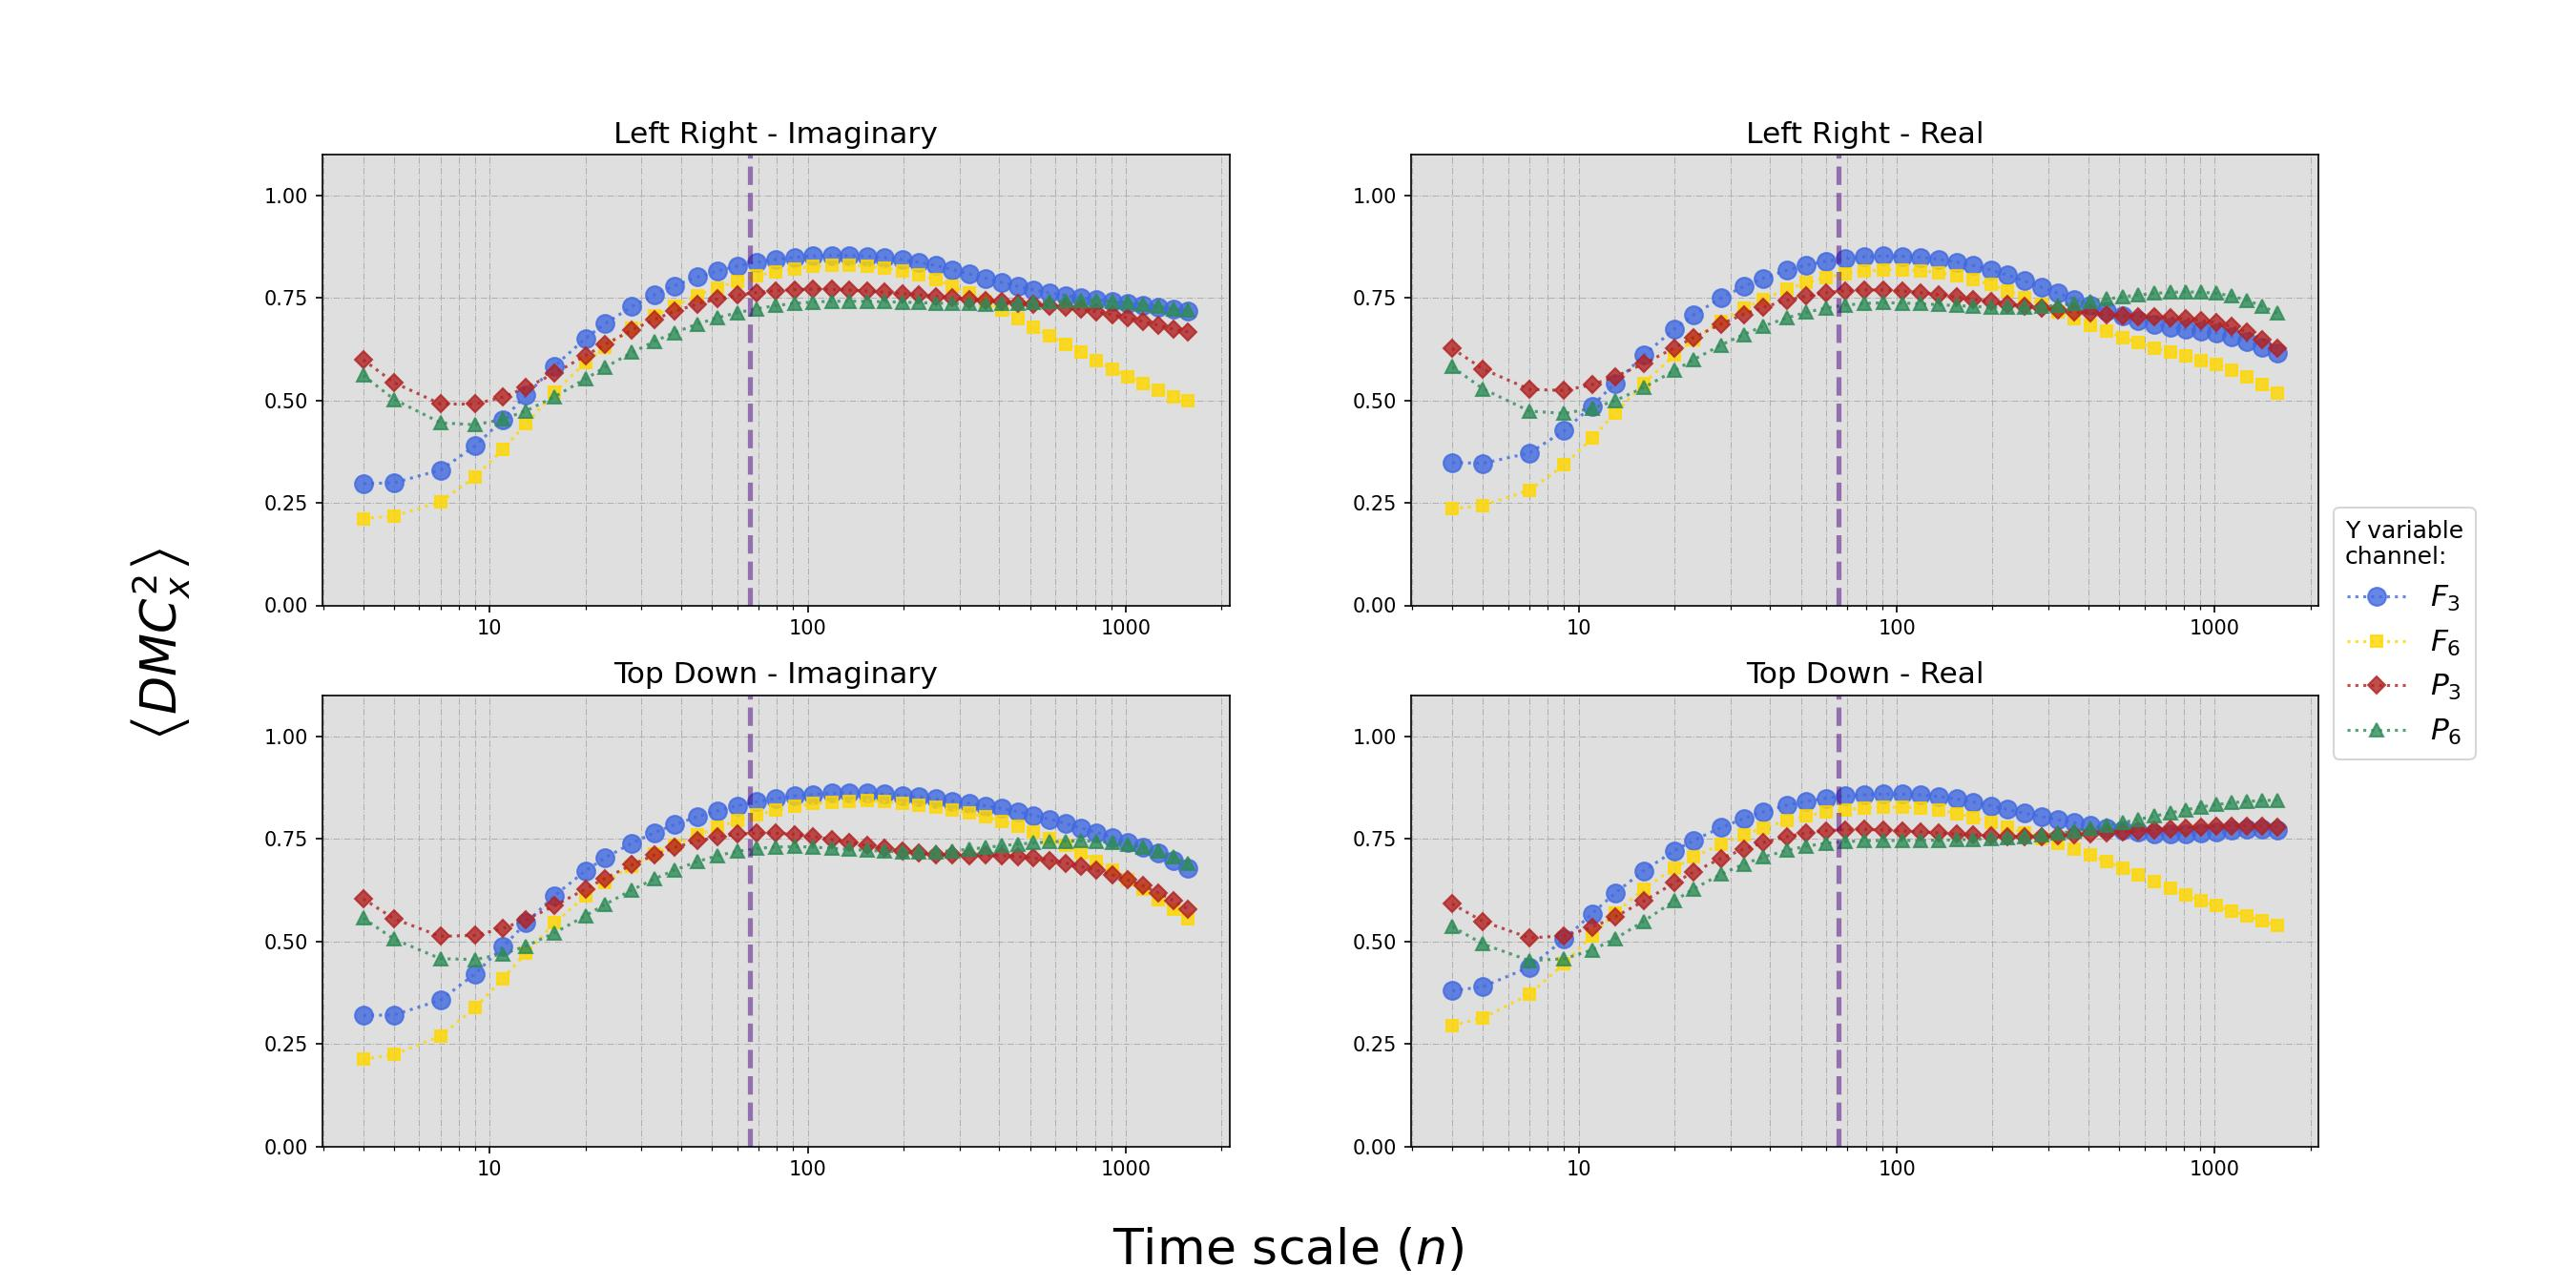
\includegraphics[height=.5\paperheight]{../Figures/art_02/Fig5.jpg}
    \caption{Mean values of $DMC_{x}^{2} \times n$ for all Tasks: Left/Right (Imaginary), Left/Right (Real), Top/Down (Imaginary), and Top/Down (Real) for the S039 subject.}
    \label{fig05}
  \end{figure}
  %%%%%%%%%%%%%%%%%%%
\end{frame}


\begin{frame}
  \frametitle{Artigo 02}

  %%%%%s%art_02/%%%%%%%%%%%%%
  \begin{figure}[!h]
    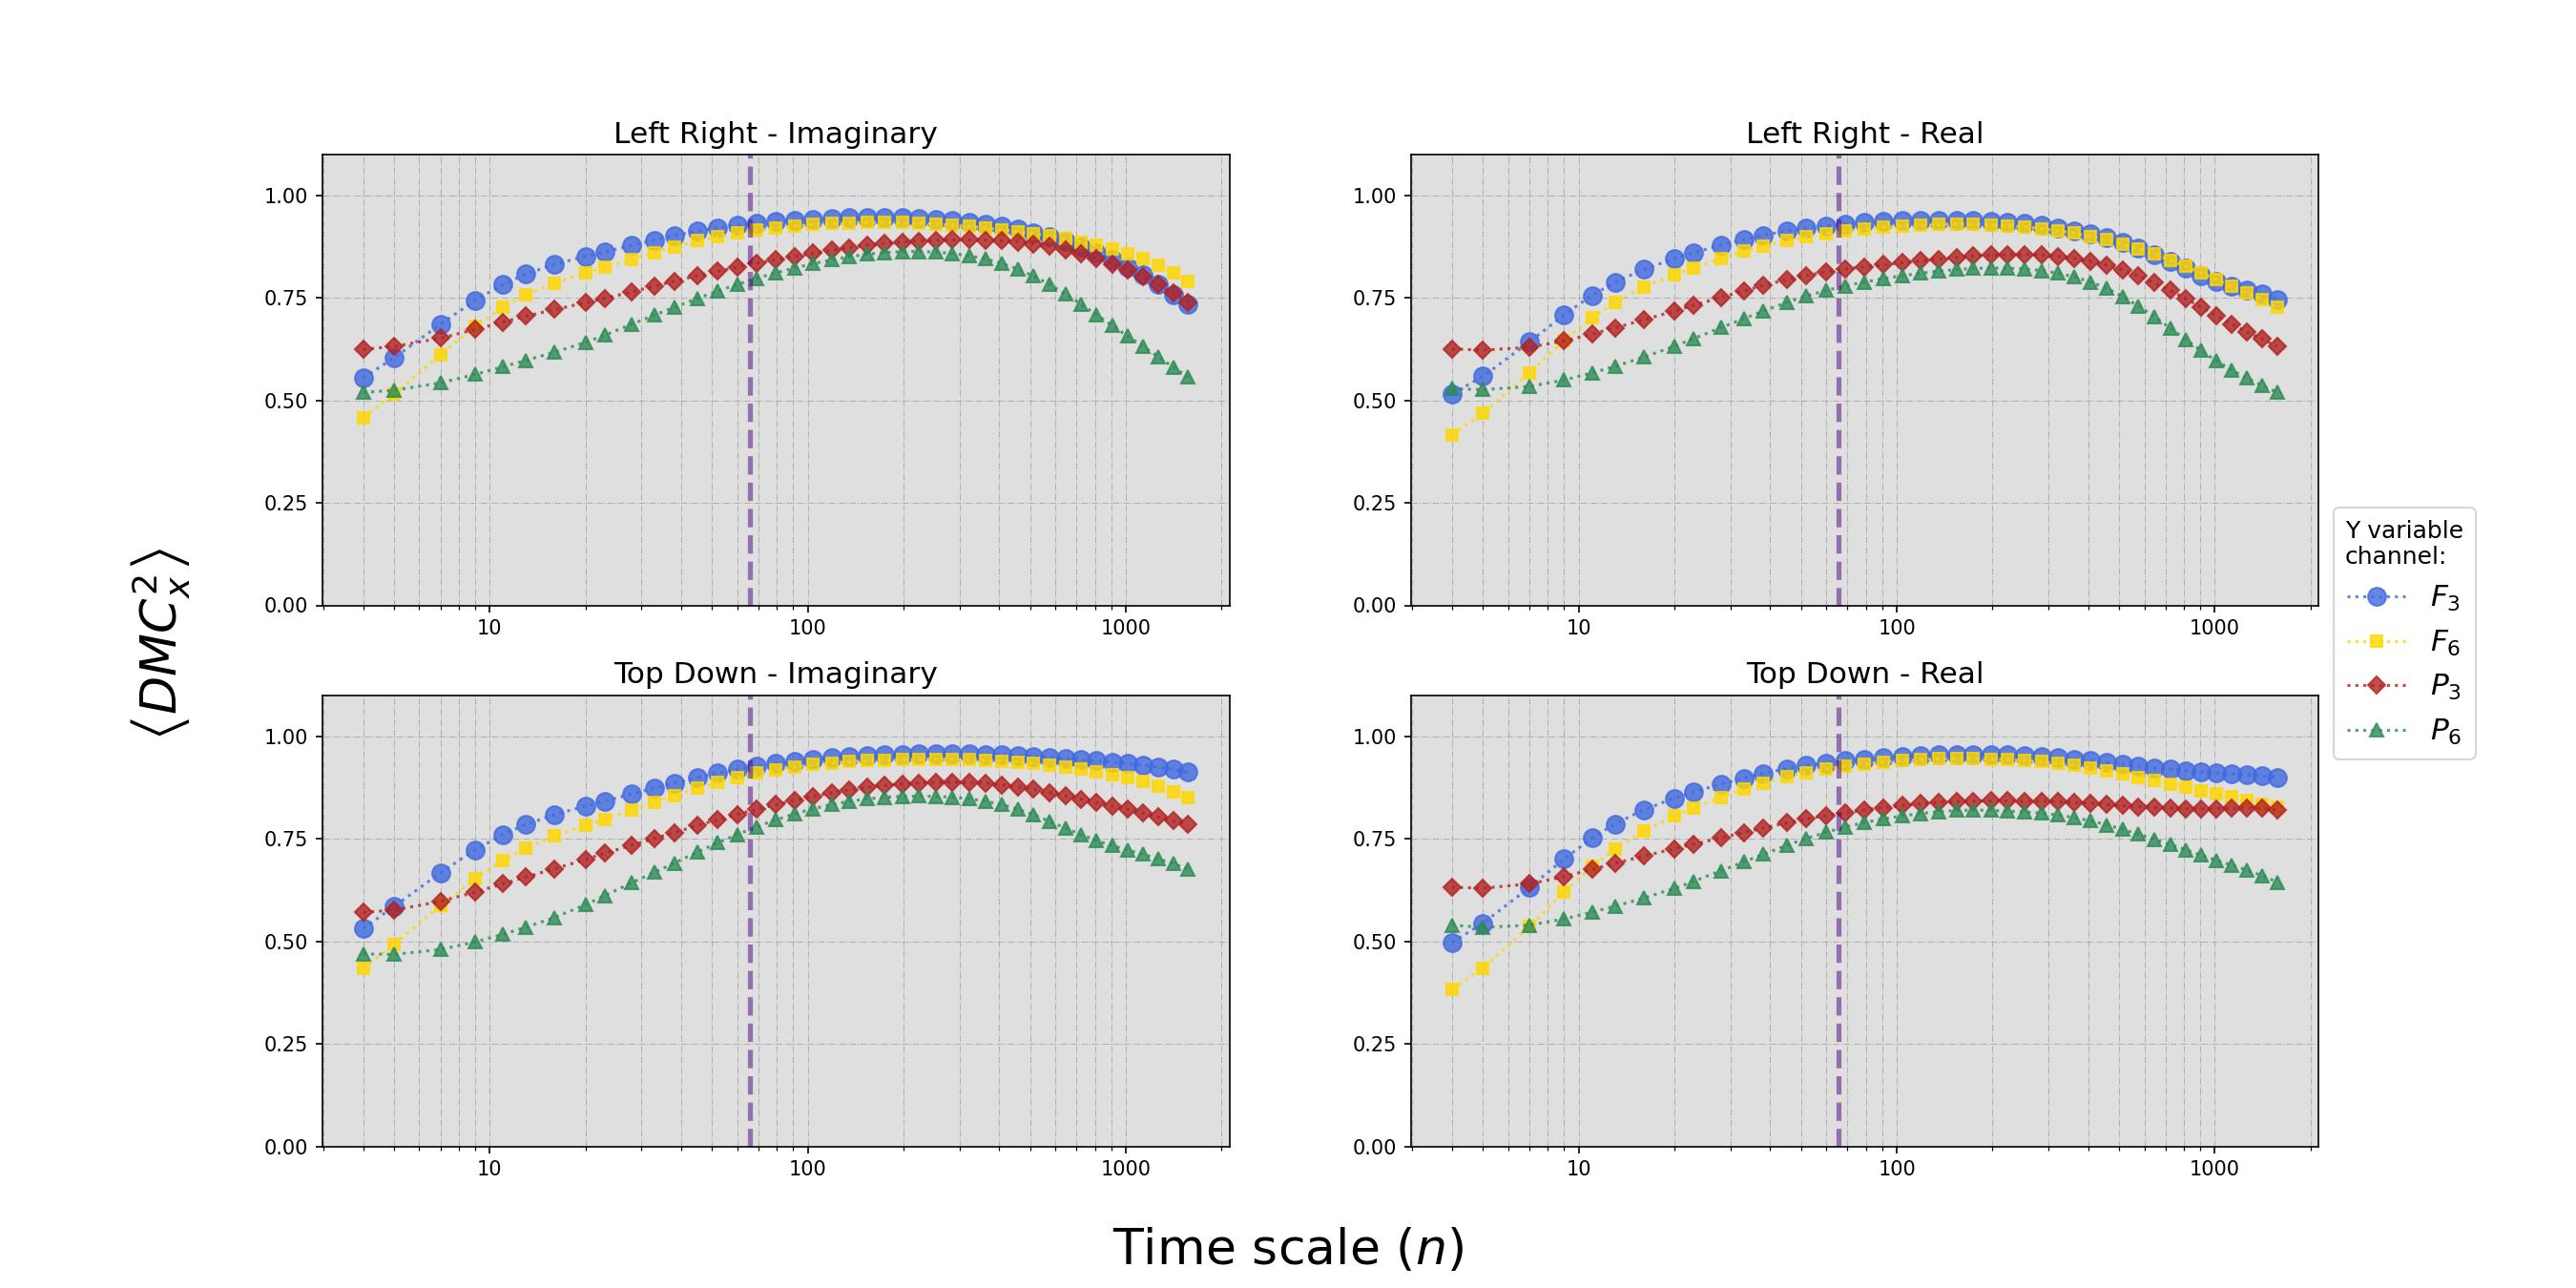
\includegraphics[height=.5\paperheight]{../Figures/art_02/Fig6.jpg}
    \caption{Mean values of $DMC_{x}^{2} \times n$ for all Tasks: Left/Right (Imaginary), Left/Right (Real), Top/Down (Imaginary), and Top/Down (Real) for the S078 subject.}
    \label{fig06}
  \end{figure}
  %%%%%%%%%%%%%%%%%%%
\end{frame}

\begin{frame}
  \frametitle{Artigo 02}

  %%%%%%%%%%%%%%%%%%%
  \begin{figure}[!h]
    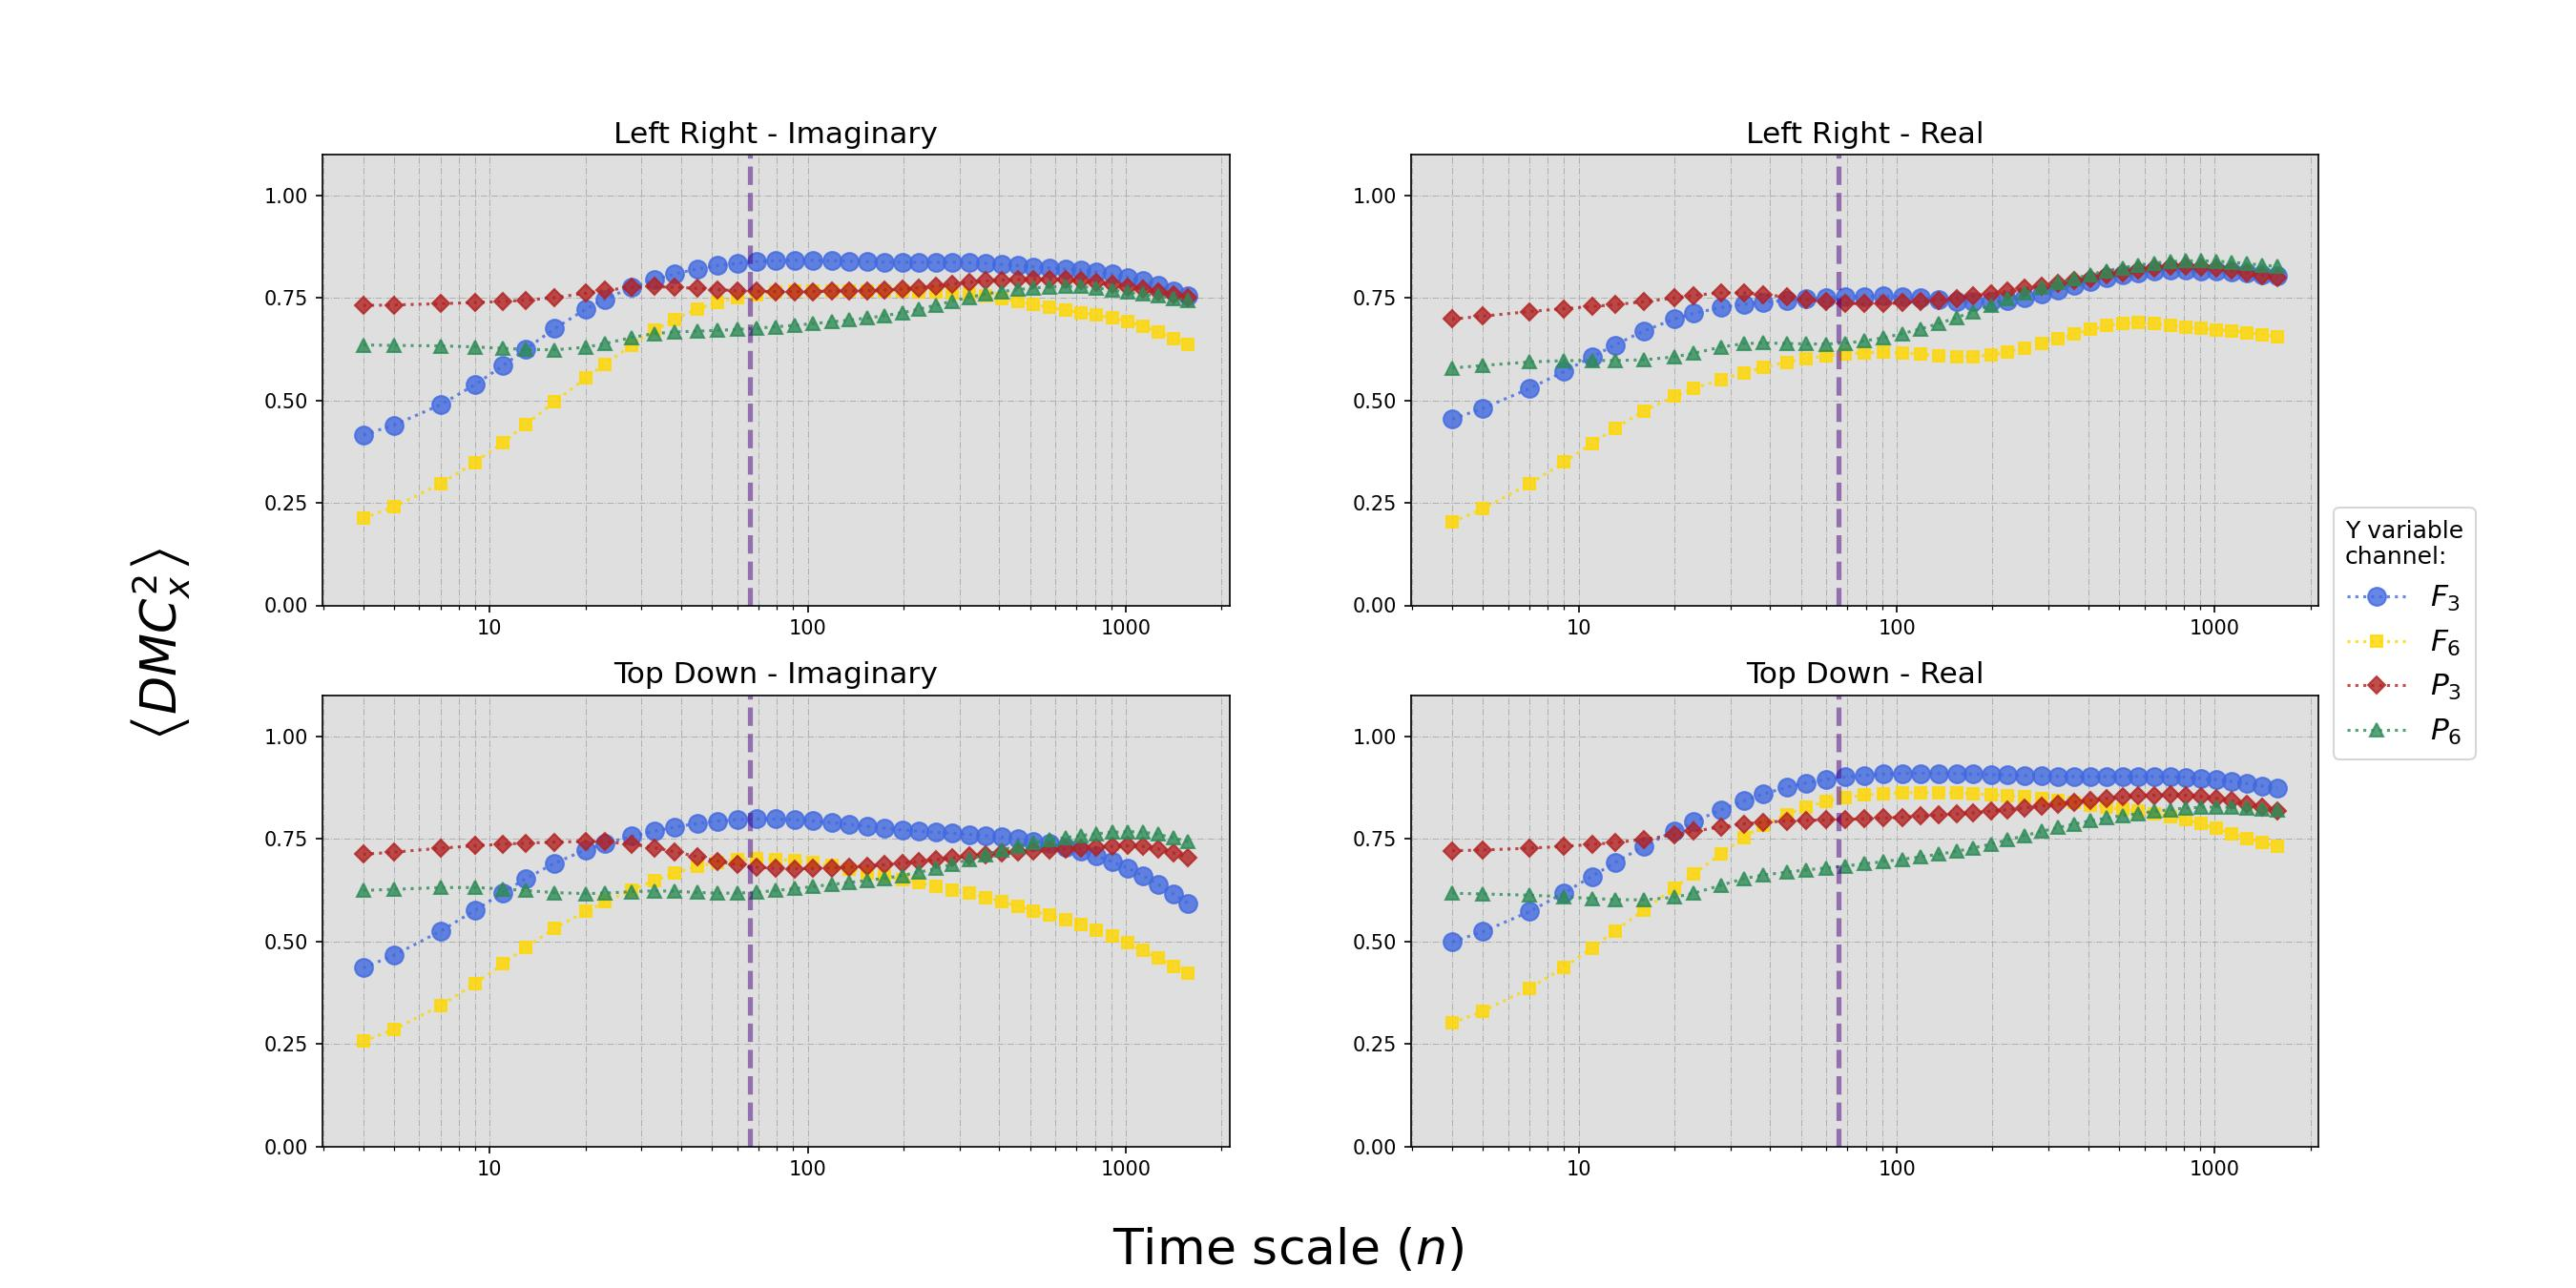
\includegraphics[height=.5\paperheight]{../Figures/art_02/Fig7.jpg}
    \caption{Mean values of $DMC_{x}^{2} \times n$ for all Tasks: Left/Right (Imaginary), Left/Right (Real), Top/Down (Imaginary), and Top/Down (Real) for the S099 subject.}
    \label{fig07}
  \end{figure}
  %%%%%%%%%%%%%%%%%%%
\end{frame}

\begin{frame}
  \frametitle{Artigo 02}

  %%%%%%%%%%%%%%%%%%%
  \begin{figure}[!h]
    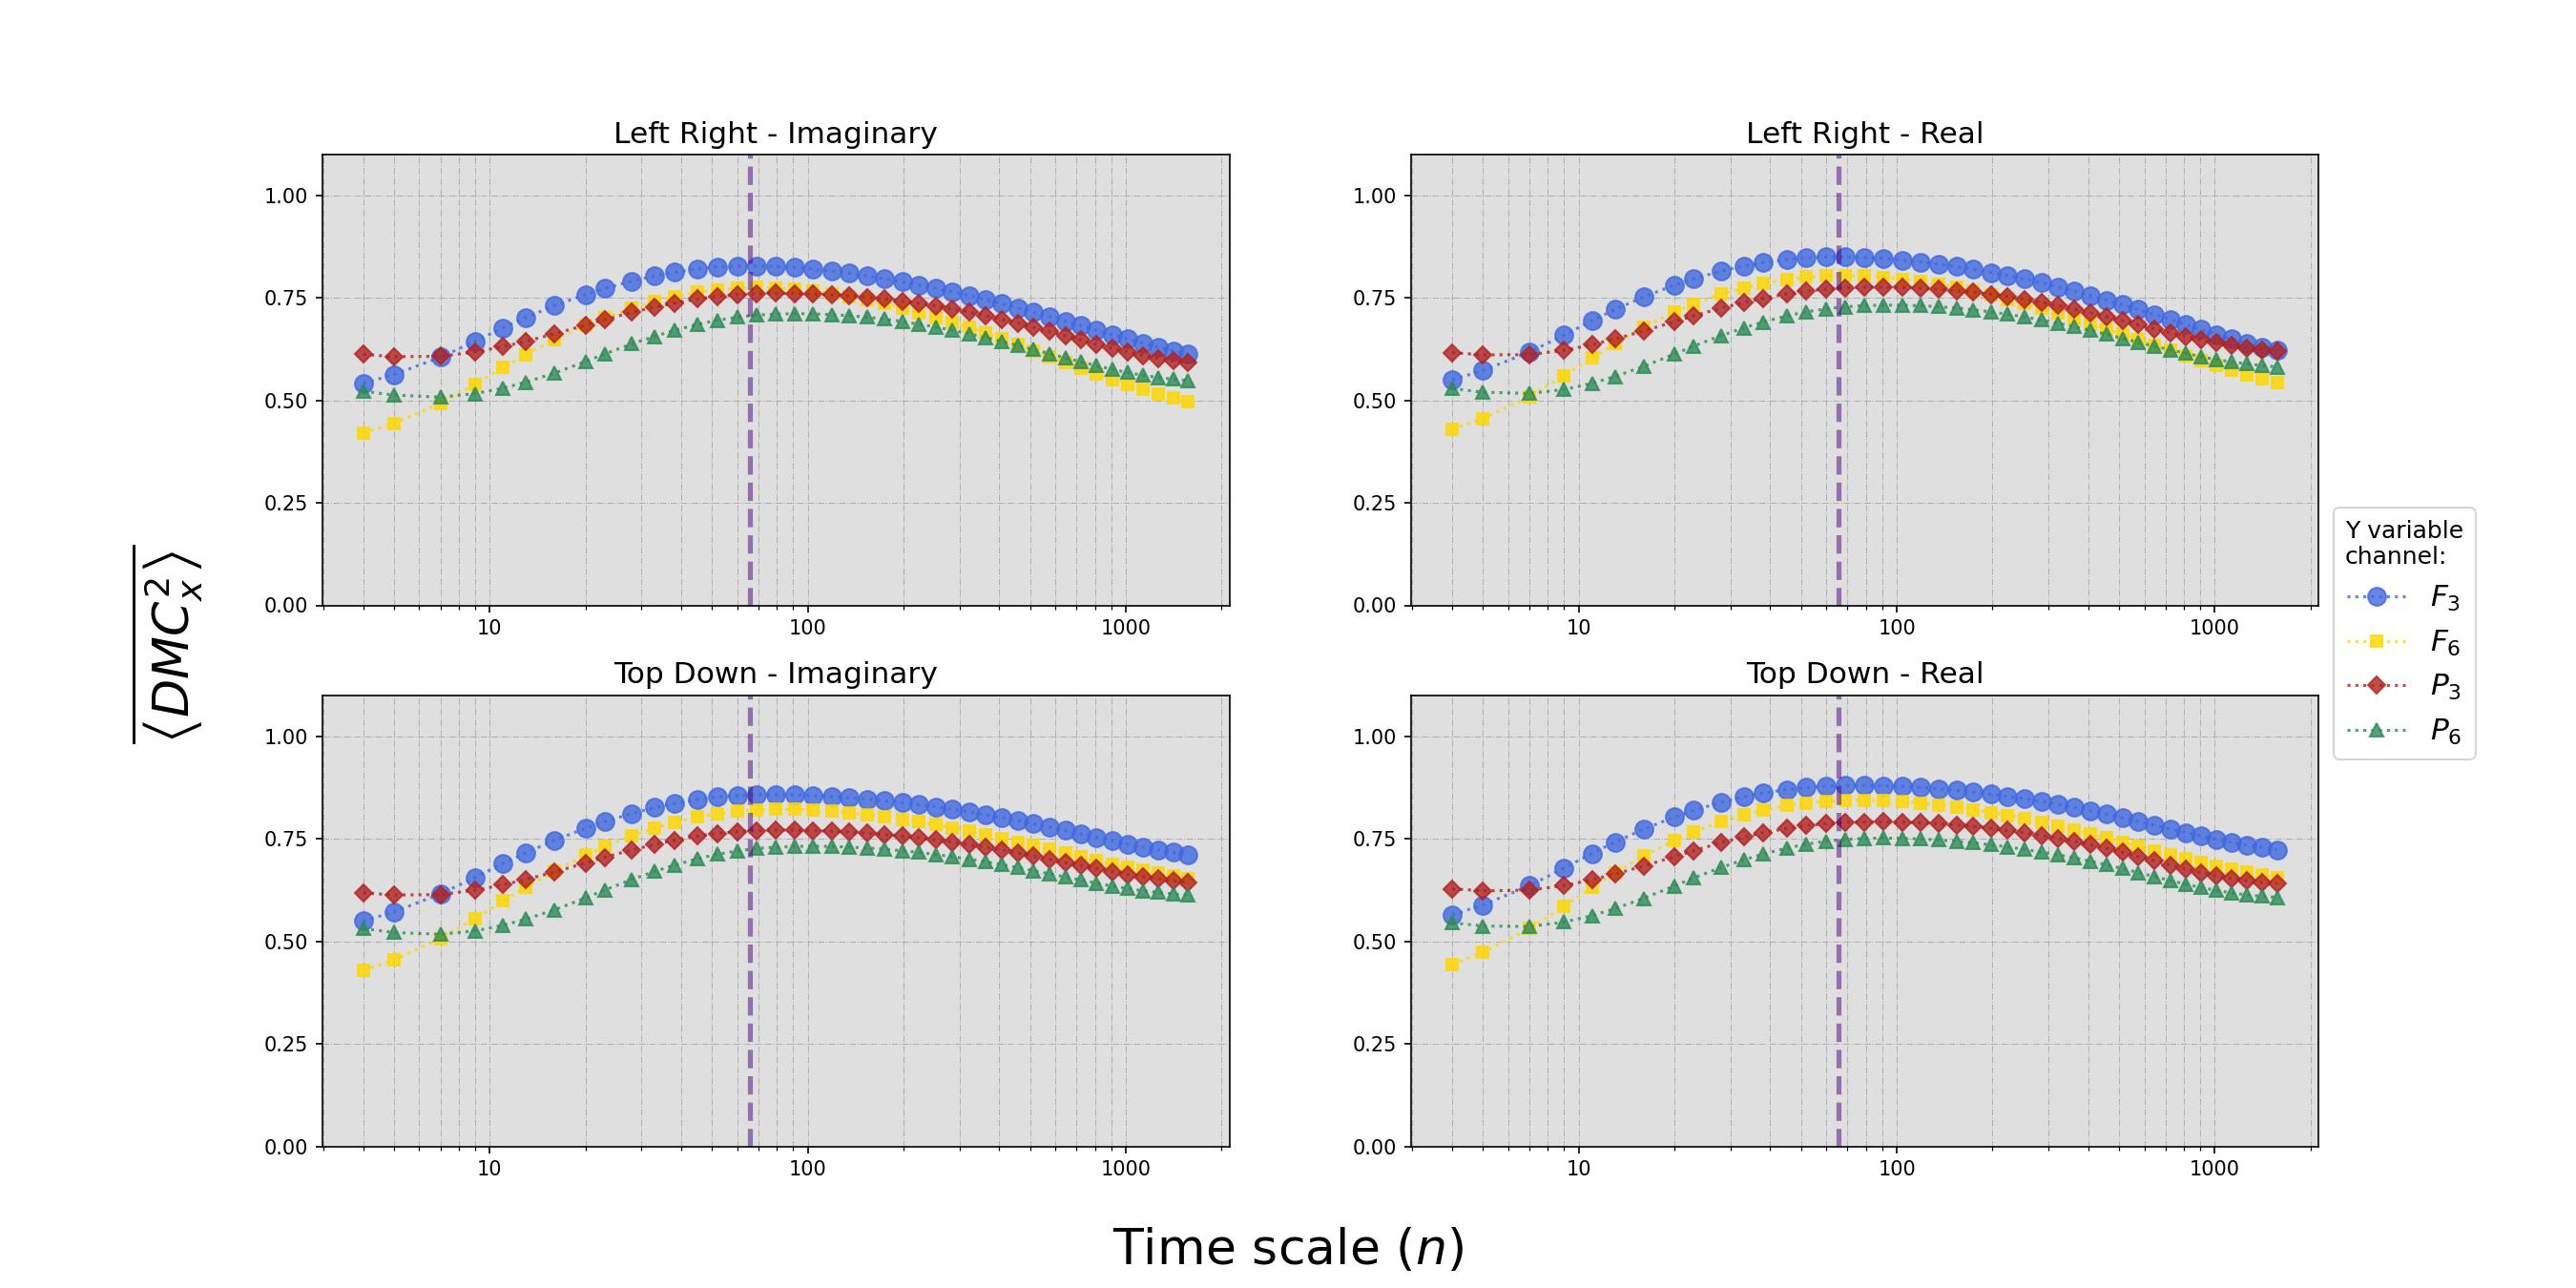
\includegraphics[height=.5\paperheight]{../Figures/art_02/Fig8.jpg}
    \caption{$DMC_{x}^{2} \times n$ mean global for all Subjects and Tasks: Left/Right (Imaginary), Left/Right (Real), Top/Down (Imaginary), and Top/Down (Real).}
    \label{fig08}
  \end{figure}
  %%%%%%%%%%%%%%%%%%%
\end{frame}


\begin{frame}
  \frametitle{Artigo 02}

  %%%%%%%%%%%%%%%%%%%
  \begin{figure}[!h]
    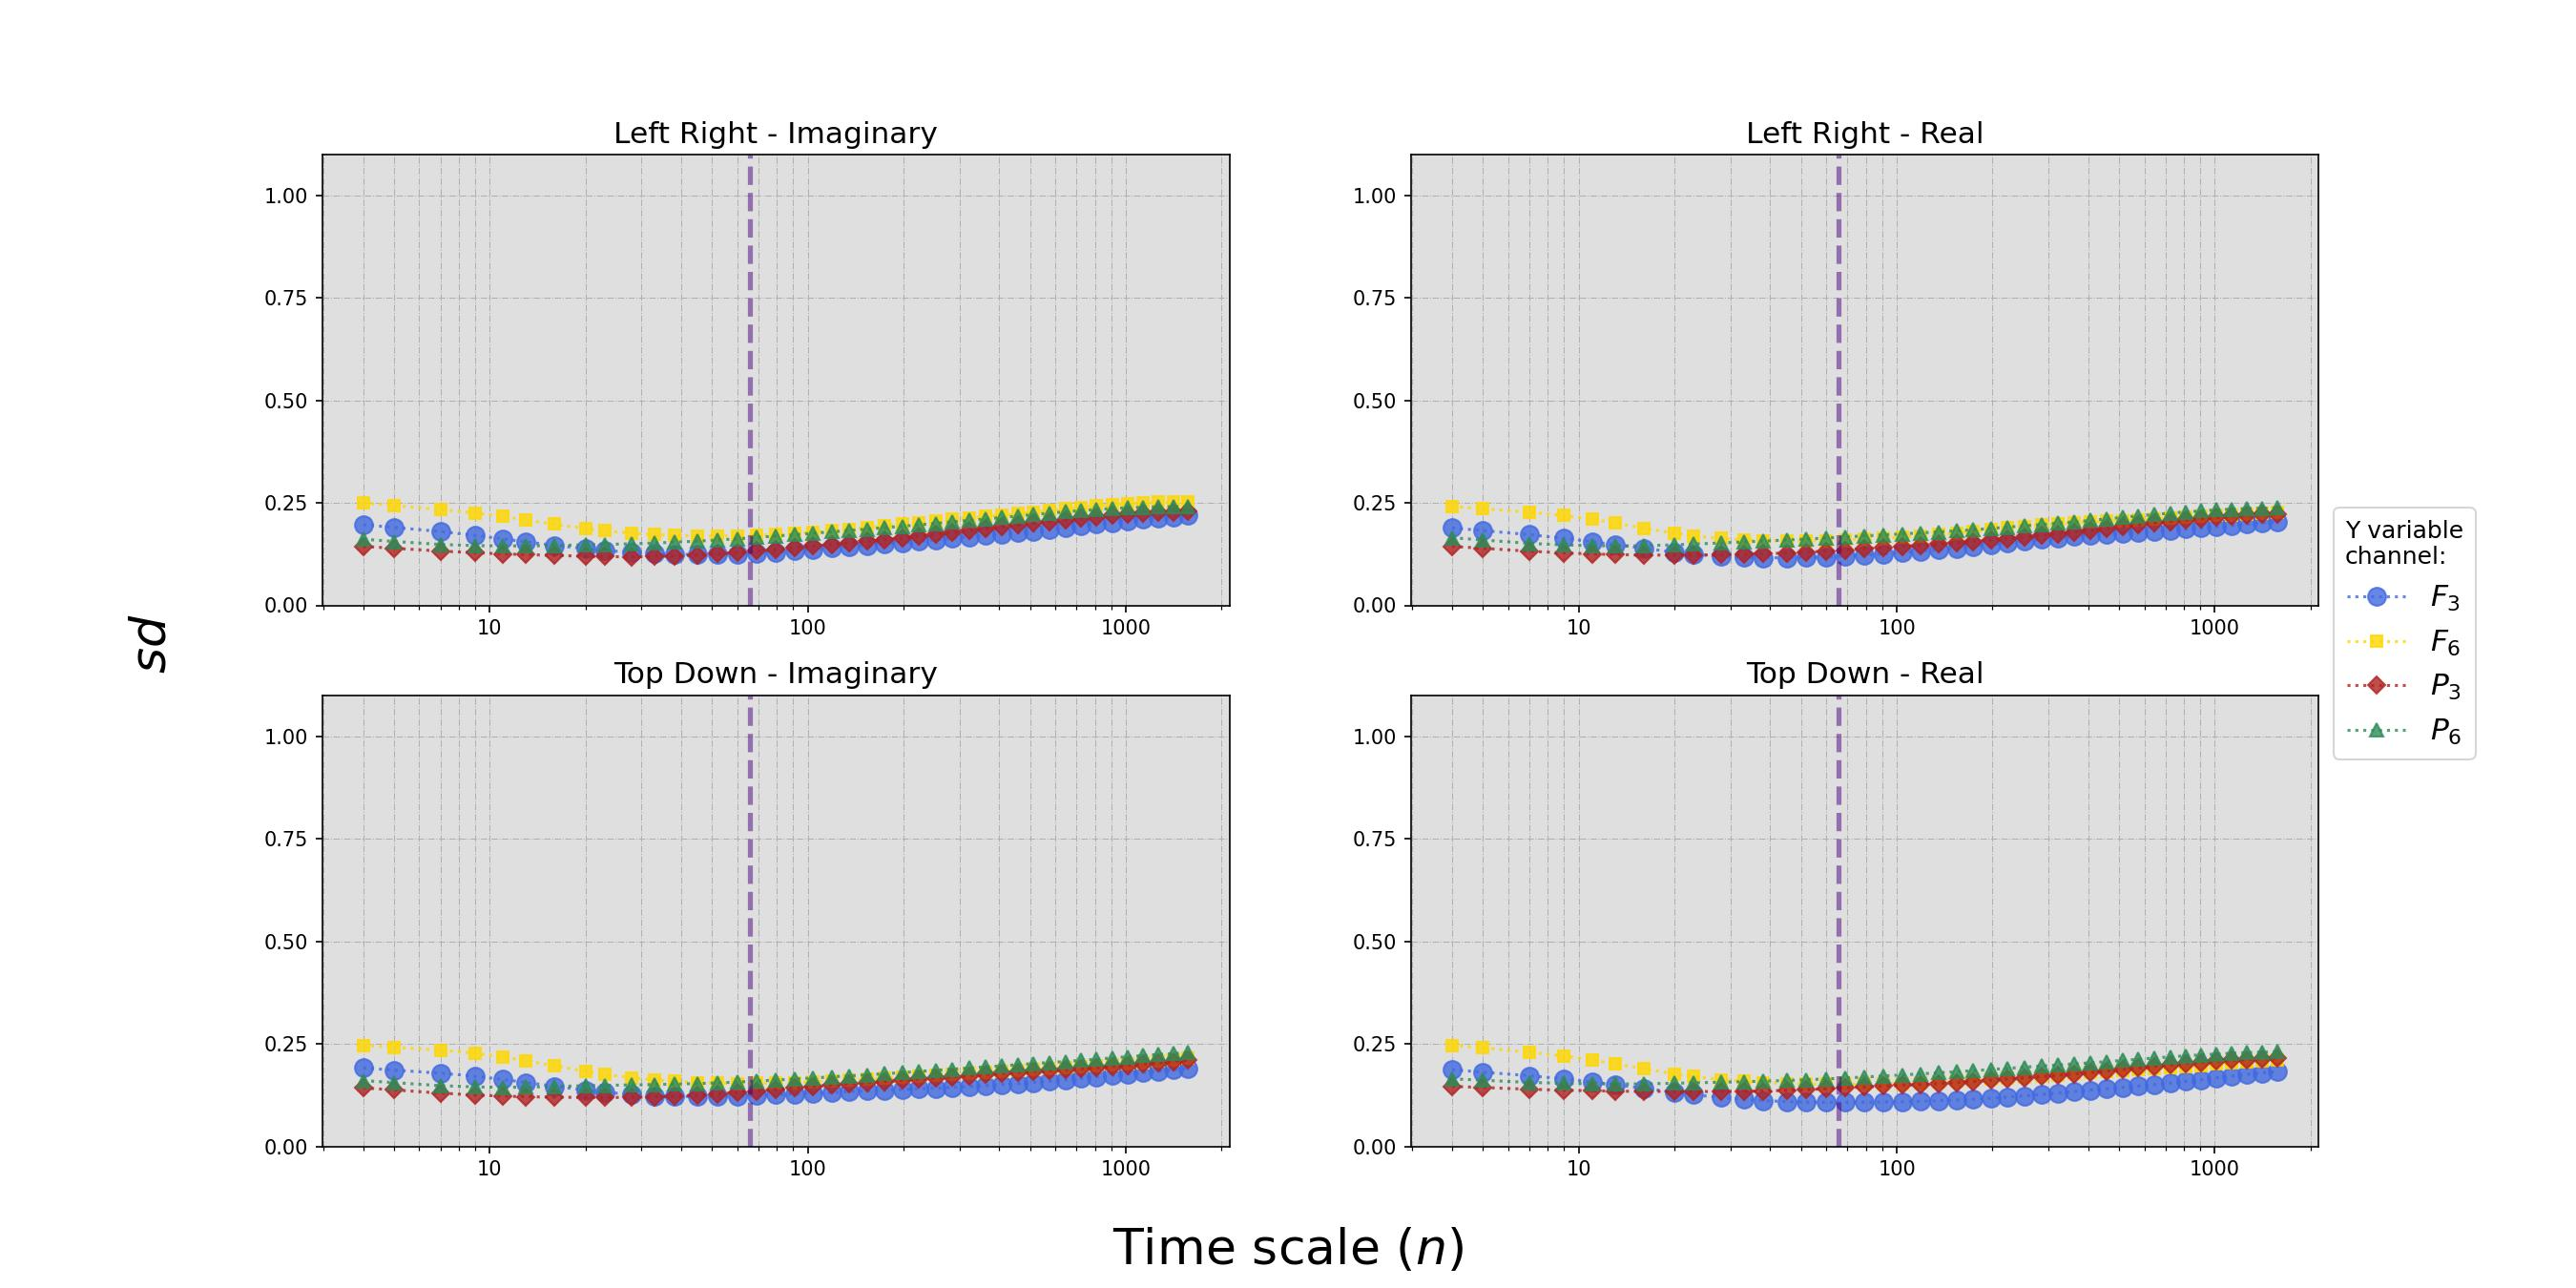
\includegraphics[height=.5\paperheight]{../Figures/art_02/Fig9.jpg}
    \caption{Standard deviation, $sd$, of the global mean for all Subjects and Tasks.}
    \label{fig09}
  \end{figure}
  %%%%%%%%%%%%%%%%%%%
\end{frame}

\begin{frame}
  \frametitle{Artigo 02}


  %%%%%%%%%%%%%%%%%%%%%%%%
  \begin{figure}[ht]
    %%%%%%%
    \begin{minipage}[b]{0.21\linewidth}
      \centering
      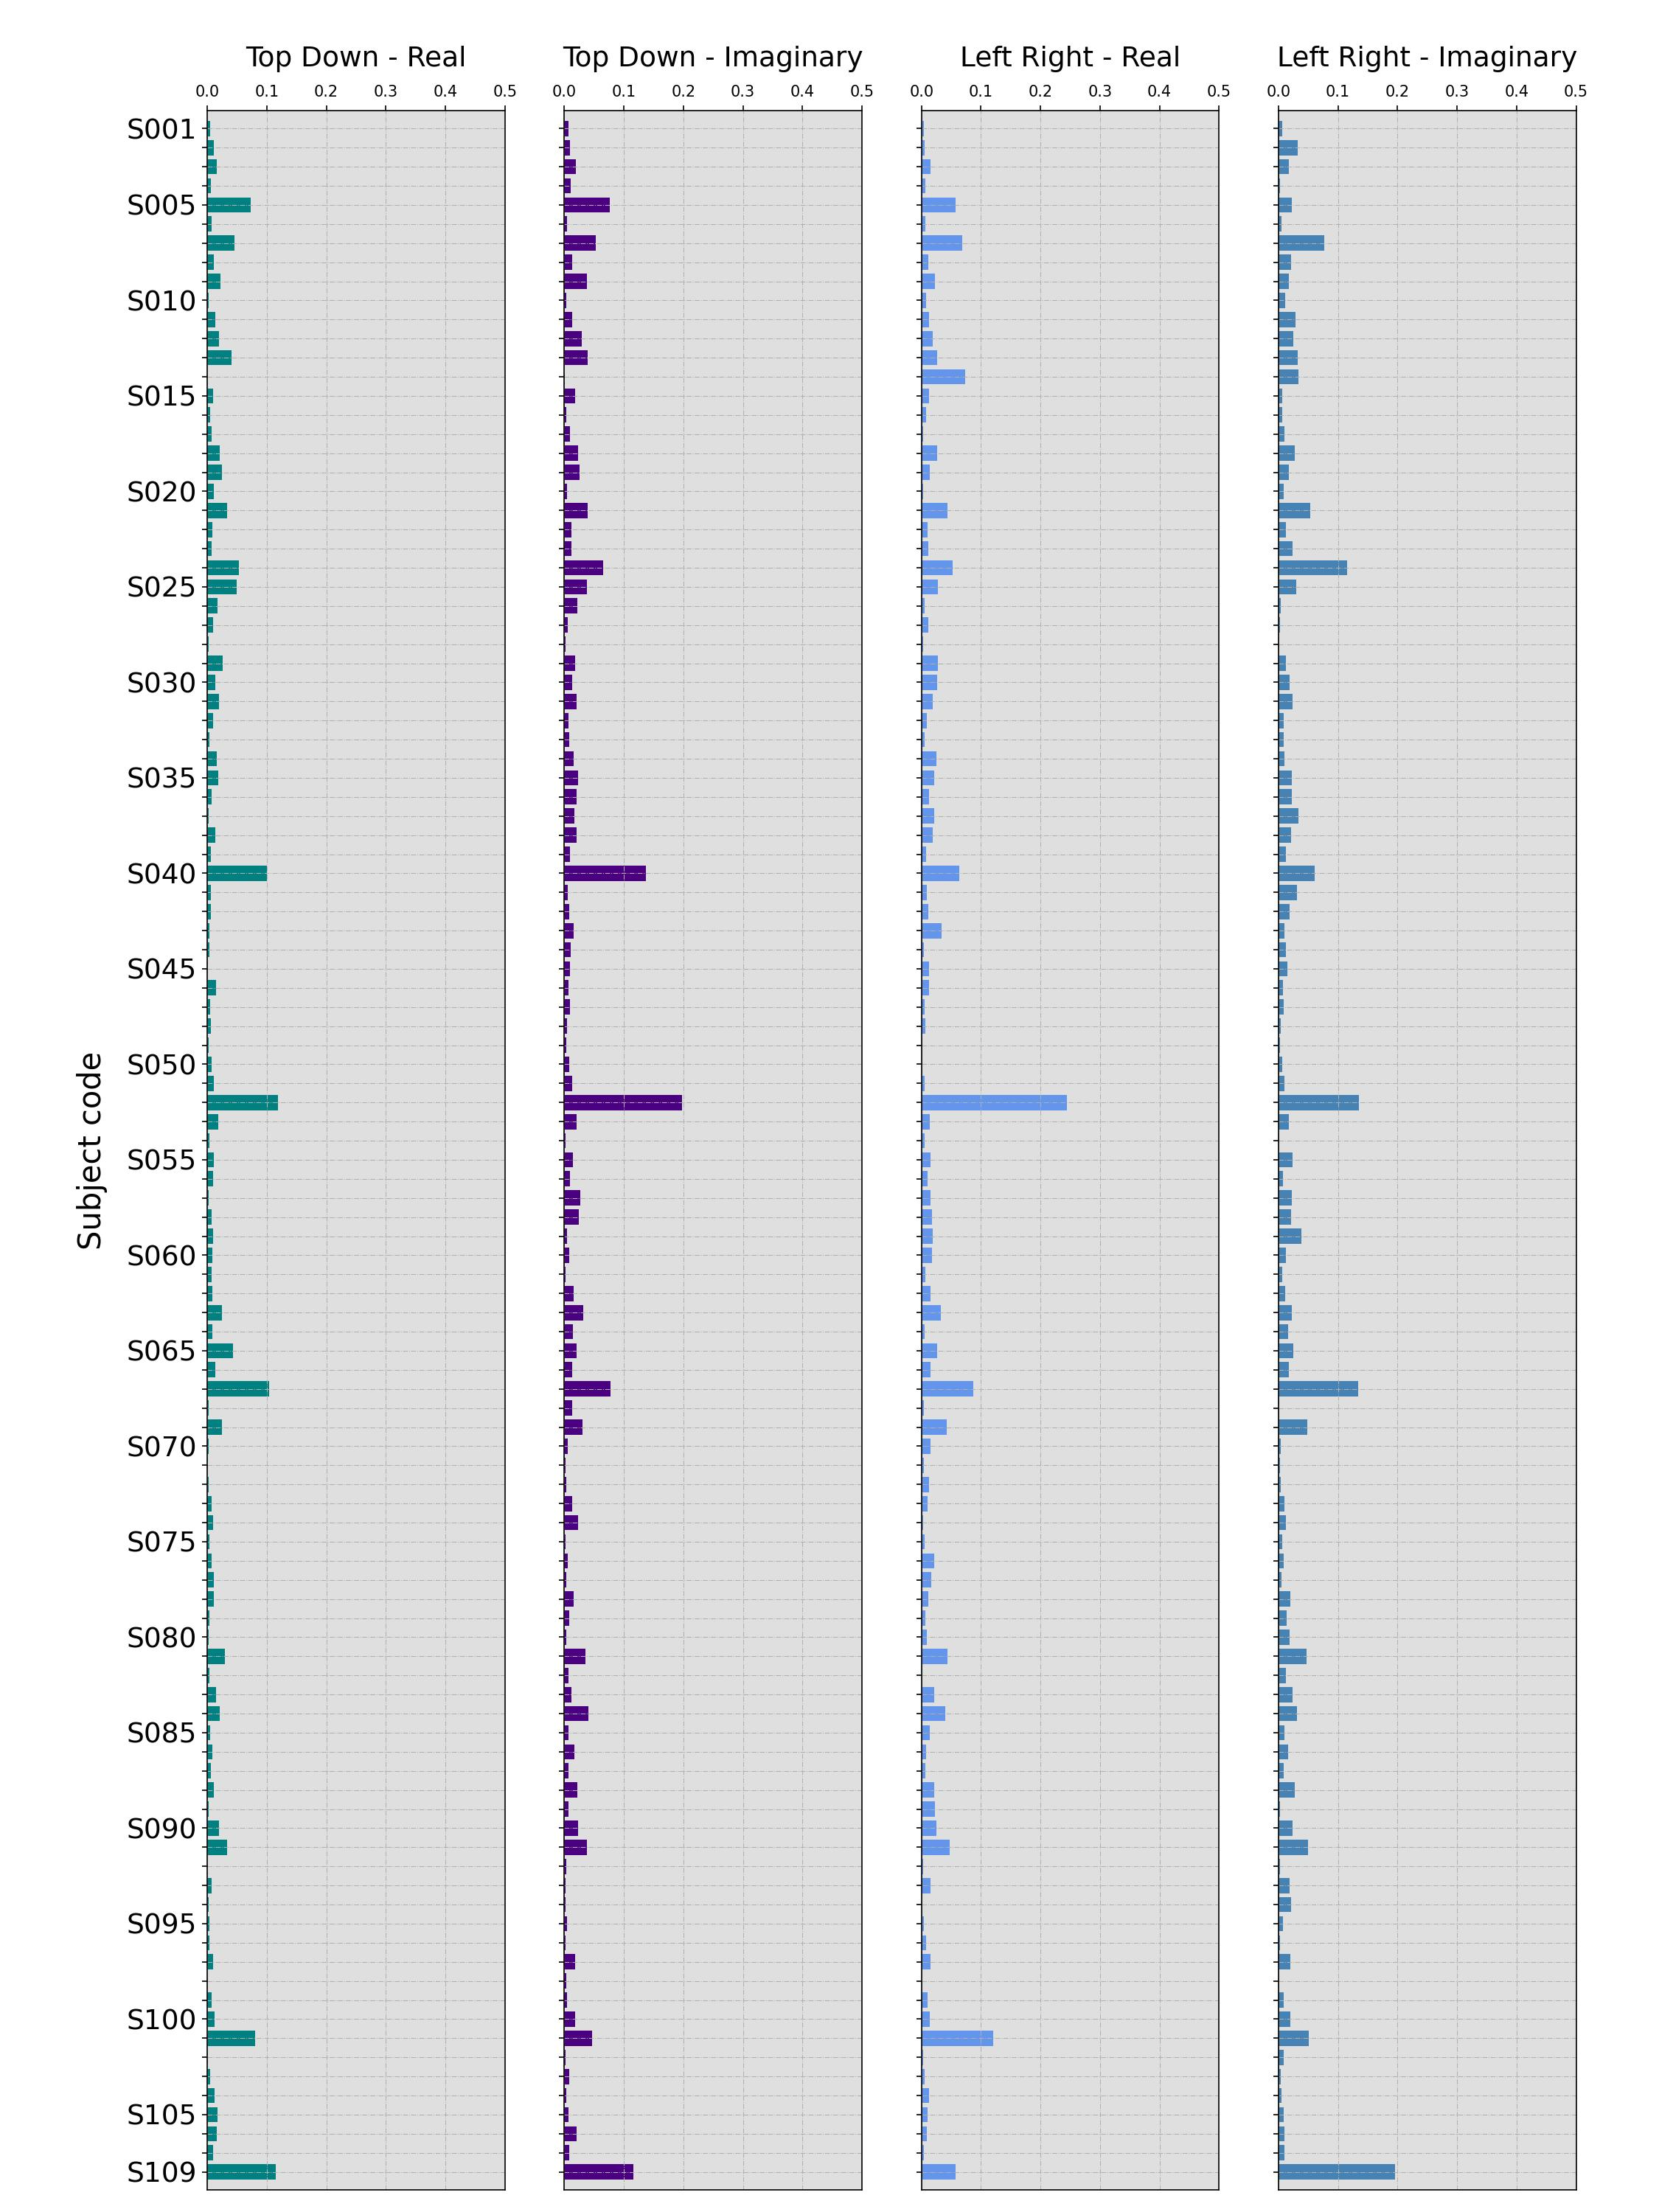
\includegraphics[height=.5\paperheight]{../Figures/art_02/Fig10.jpg}
      \caption{MSE for the Channel $F_{3}$.}
      \label{fig21}

    \end{minipage}
    %%%%%%%
    \hspace{0.2cm}
    %%%%%%%
    \begin{minipage}[b]{0.21\linewidth}
      \centering
      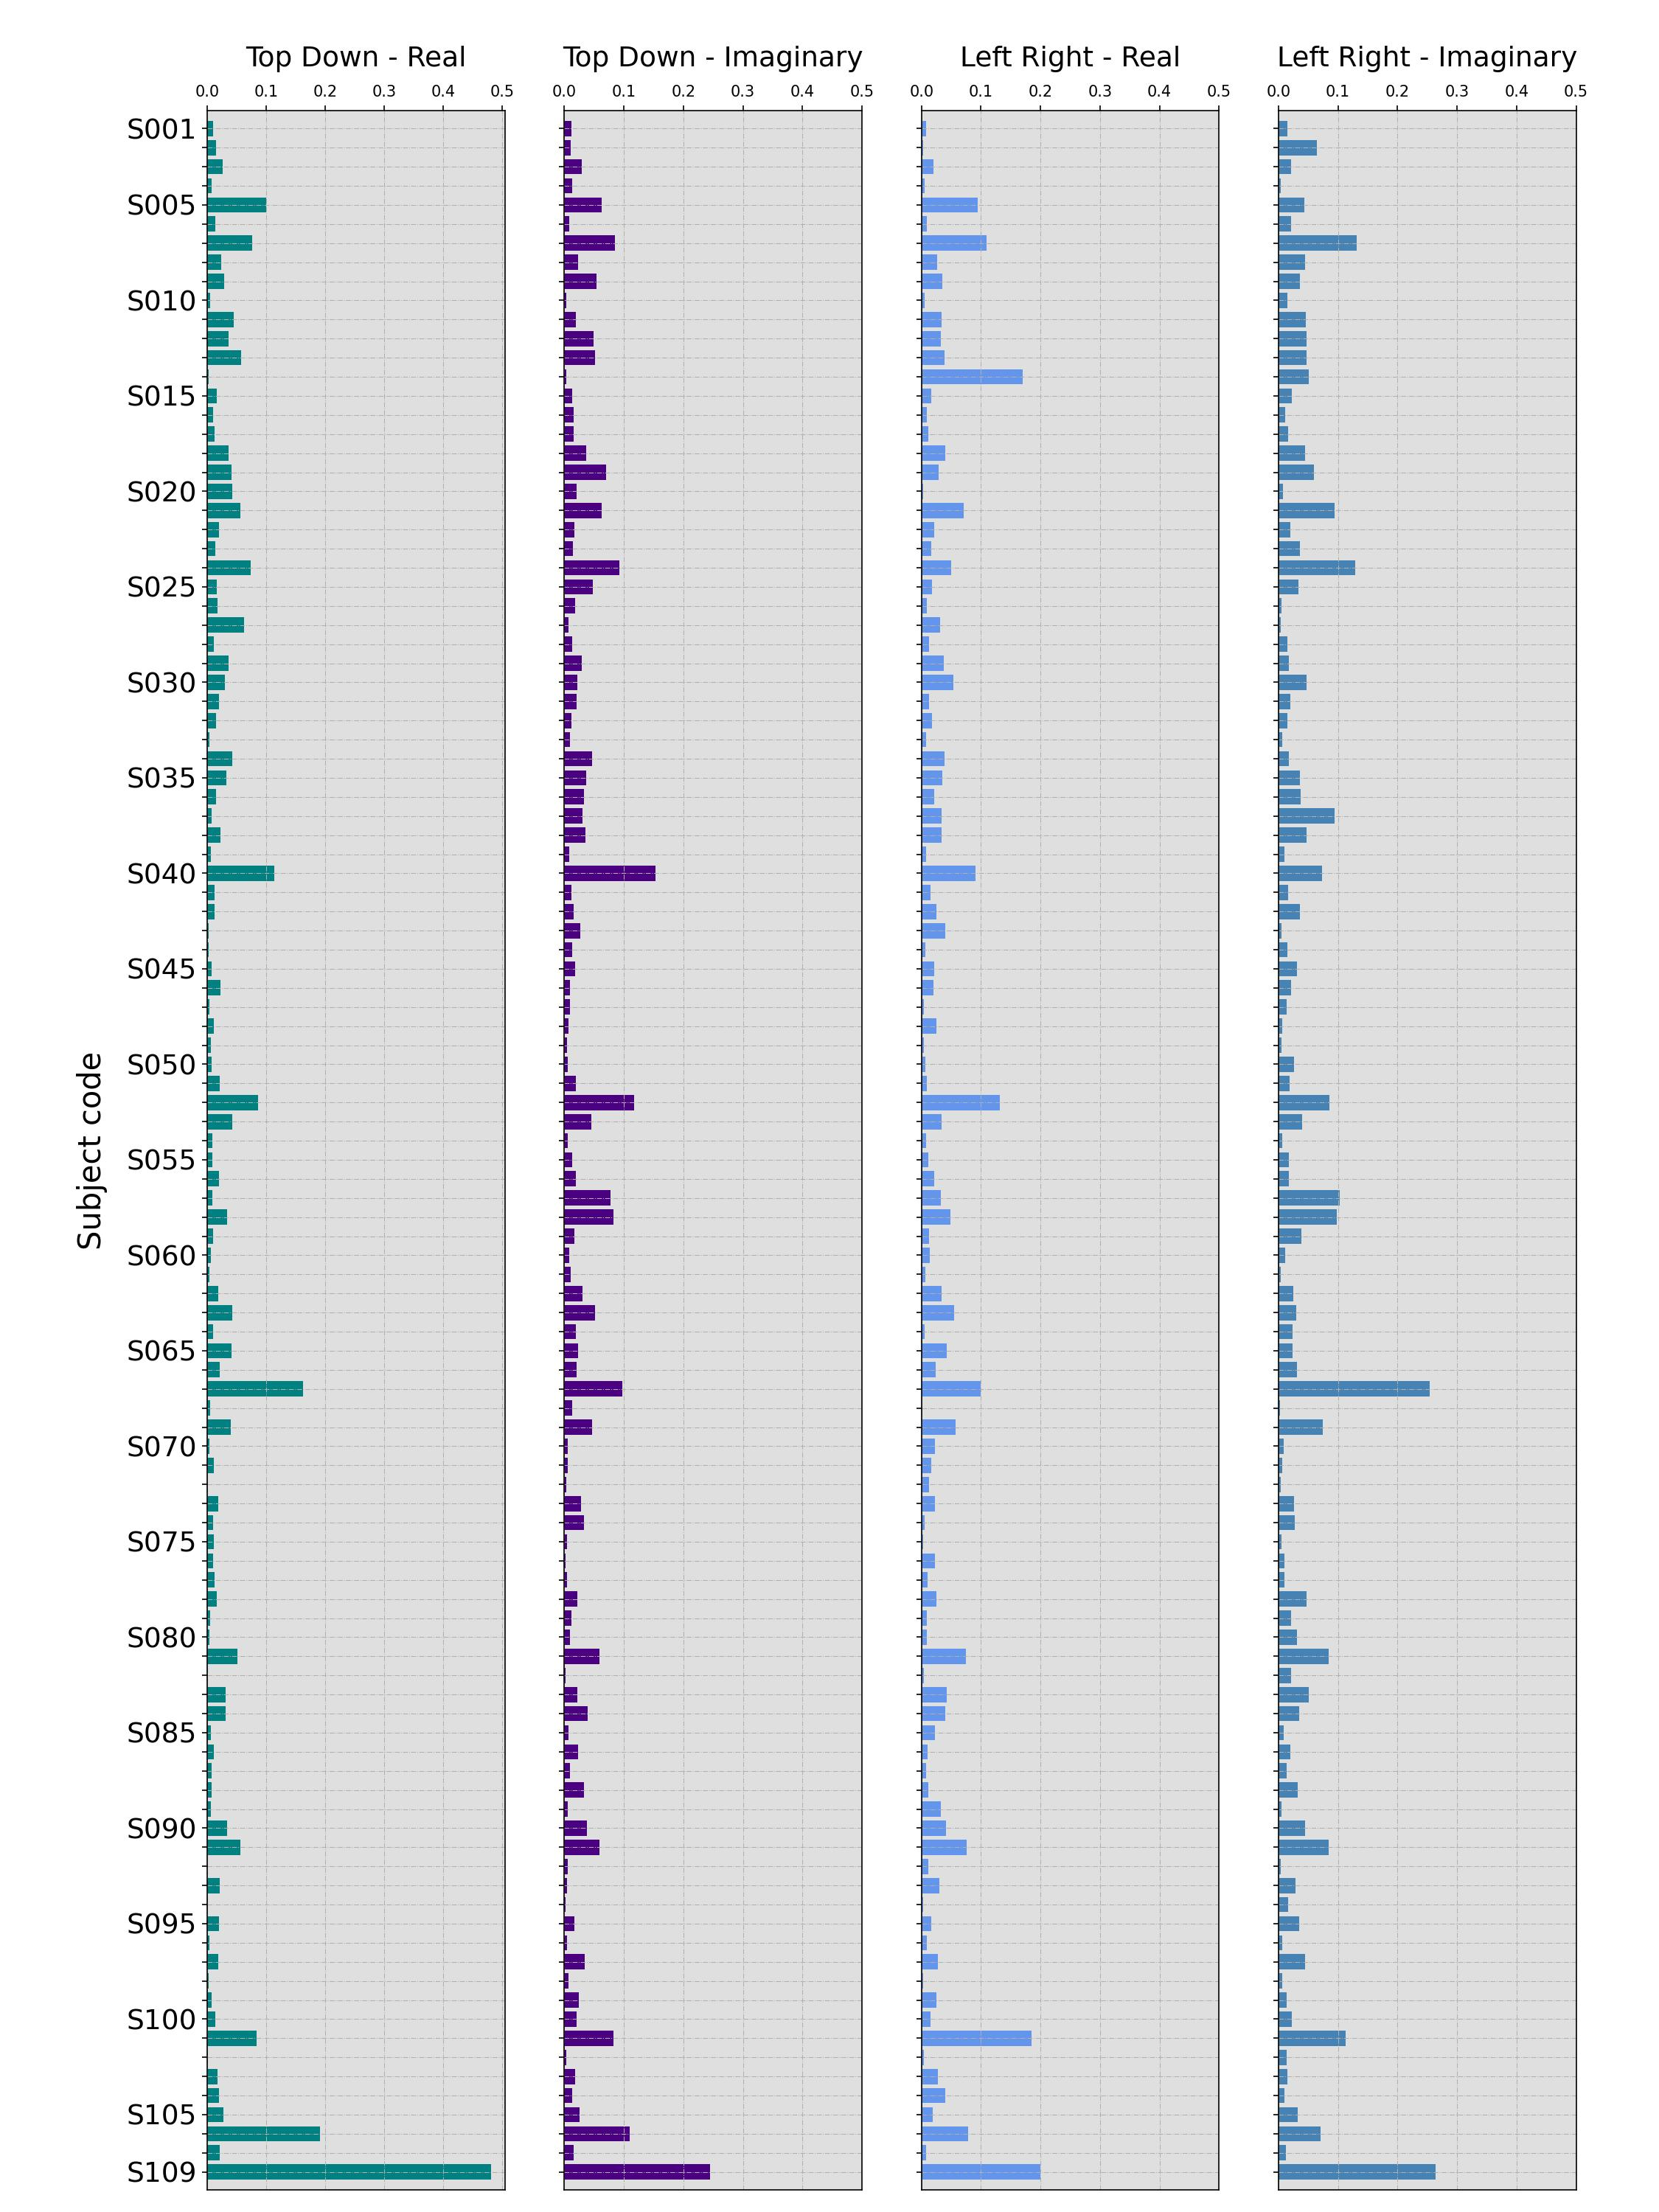
\includegraphics[height=.5\paperheight]{../Figures/art_02/Fig11.jpg}
      \caption{MSE for the Channel $F_{6}$.}
      \label{fig22}
    \end{minipage}
    %%%%%%%
    \hspace{0.2cm}
    %%%%%%%
    \begin{minipage}[b]{0.21\linewidth}
      \centering
      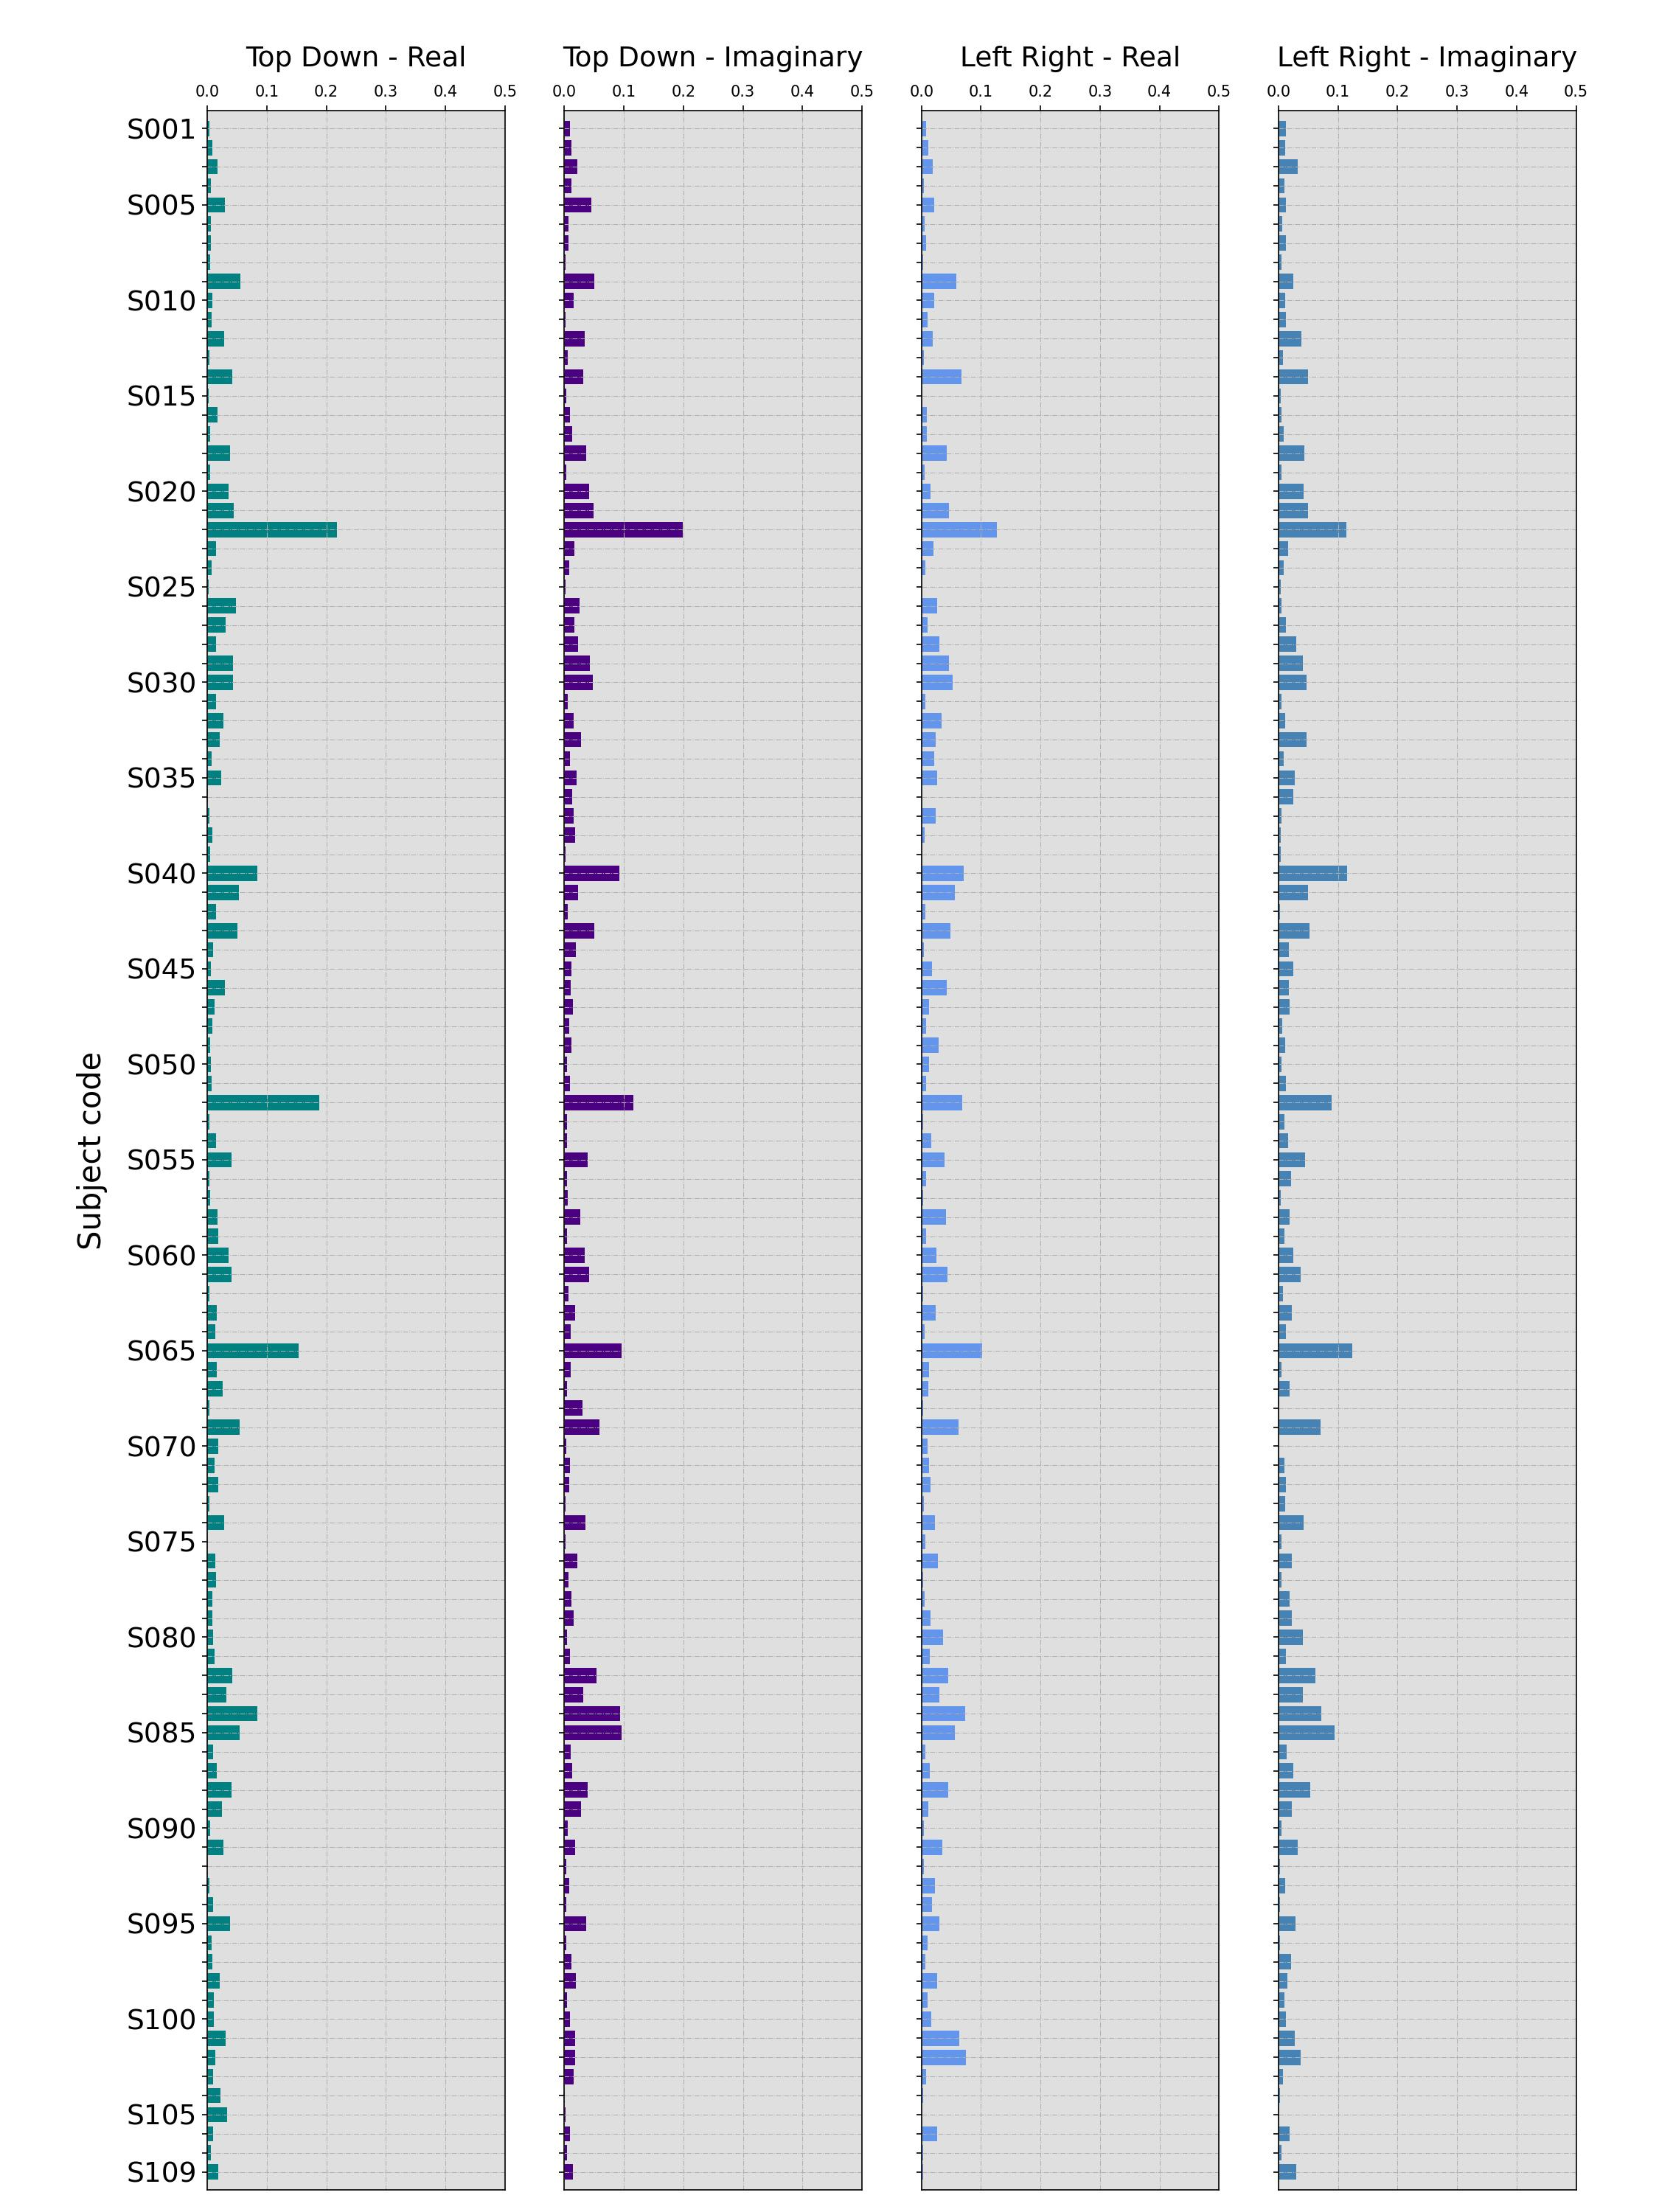
\includegraphics[height=.5\paperheight]{../Figures/art_02/Fig12.jpg}
      \caption{MSE for the Channel $P_{3}$.}
      \label{fig23}
    \end{minipage}
    %%%%%%%
    \hspace{0.2cm}
    %%%%%%%
    \begin{minipage}[b]{0.21\linewidth}
      \centering
      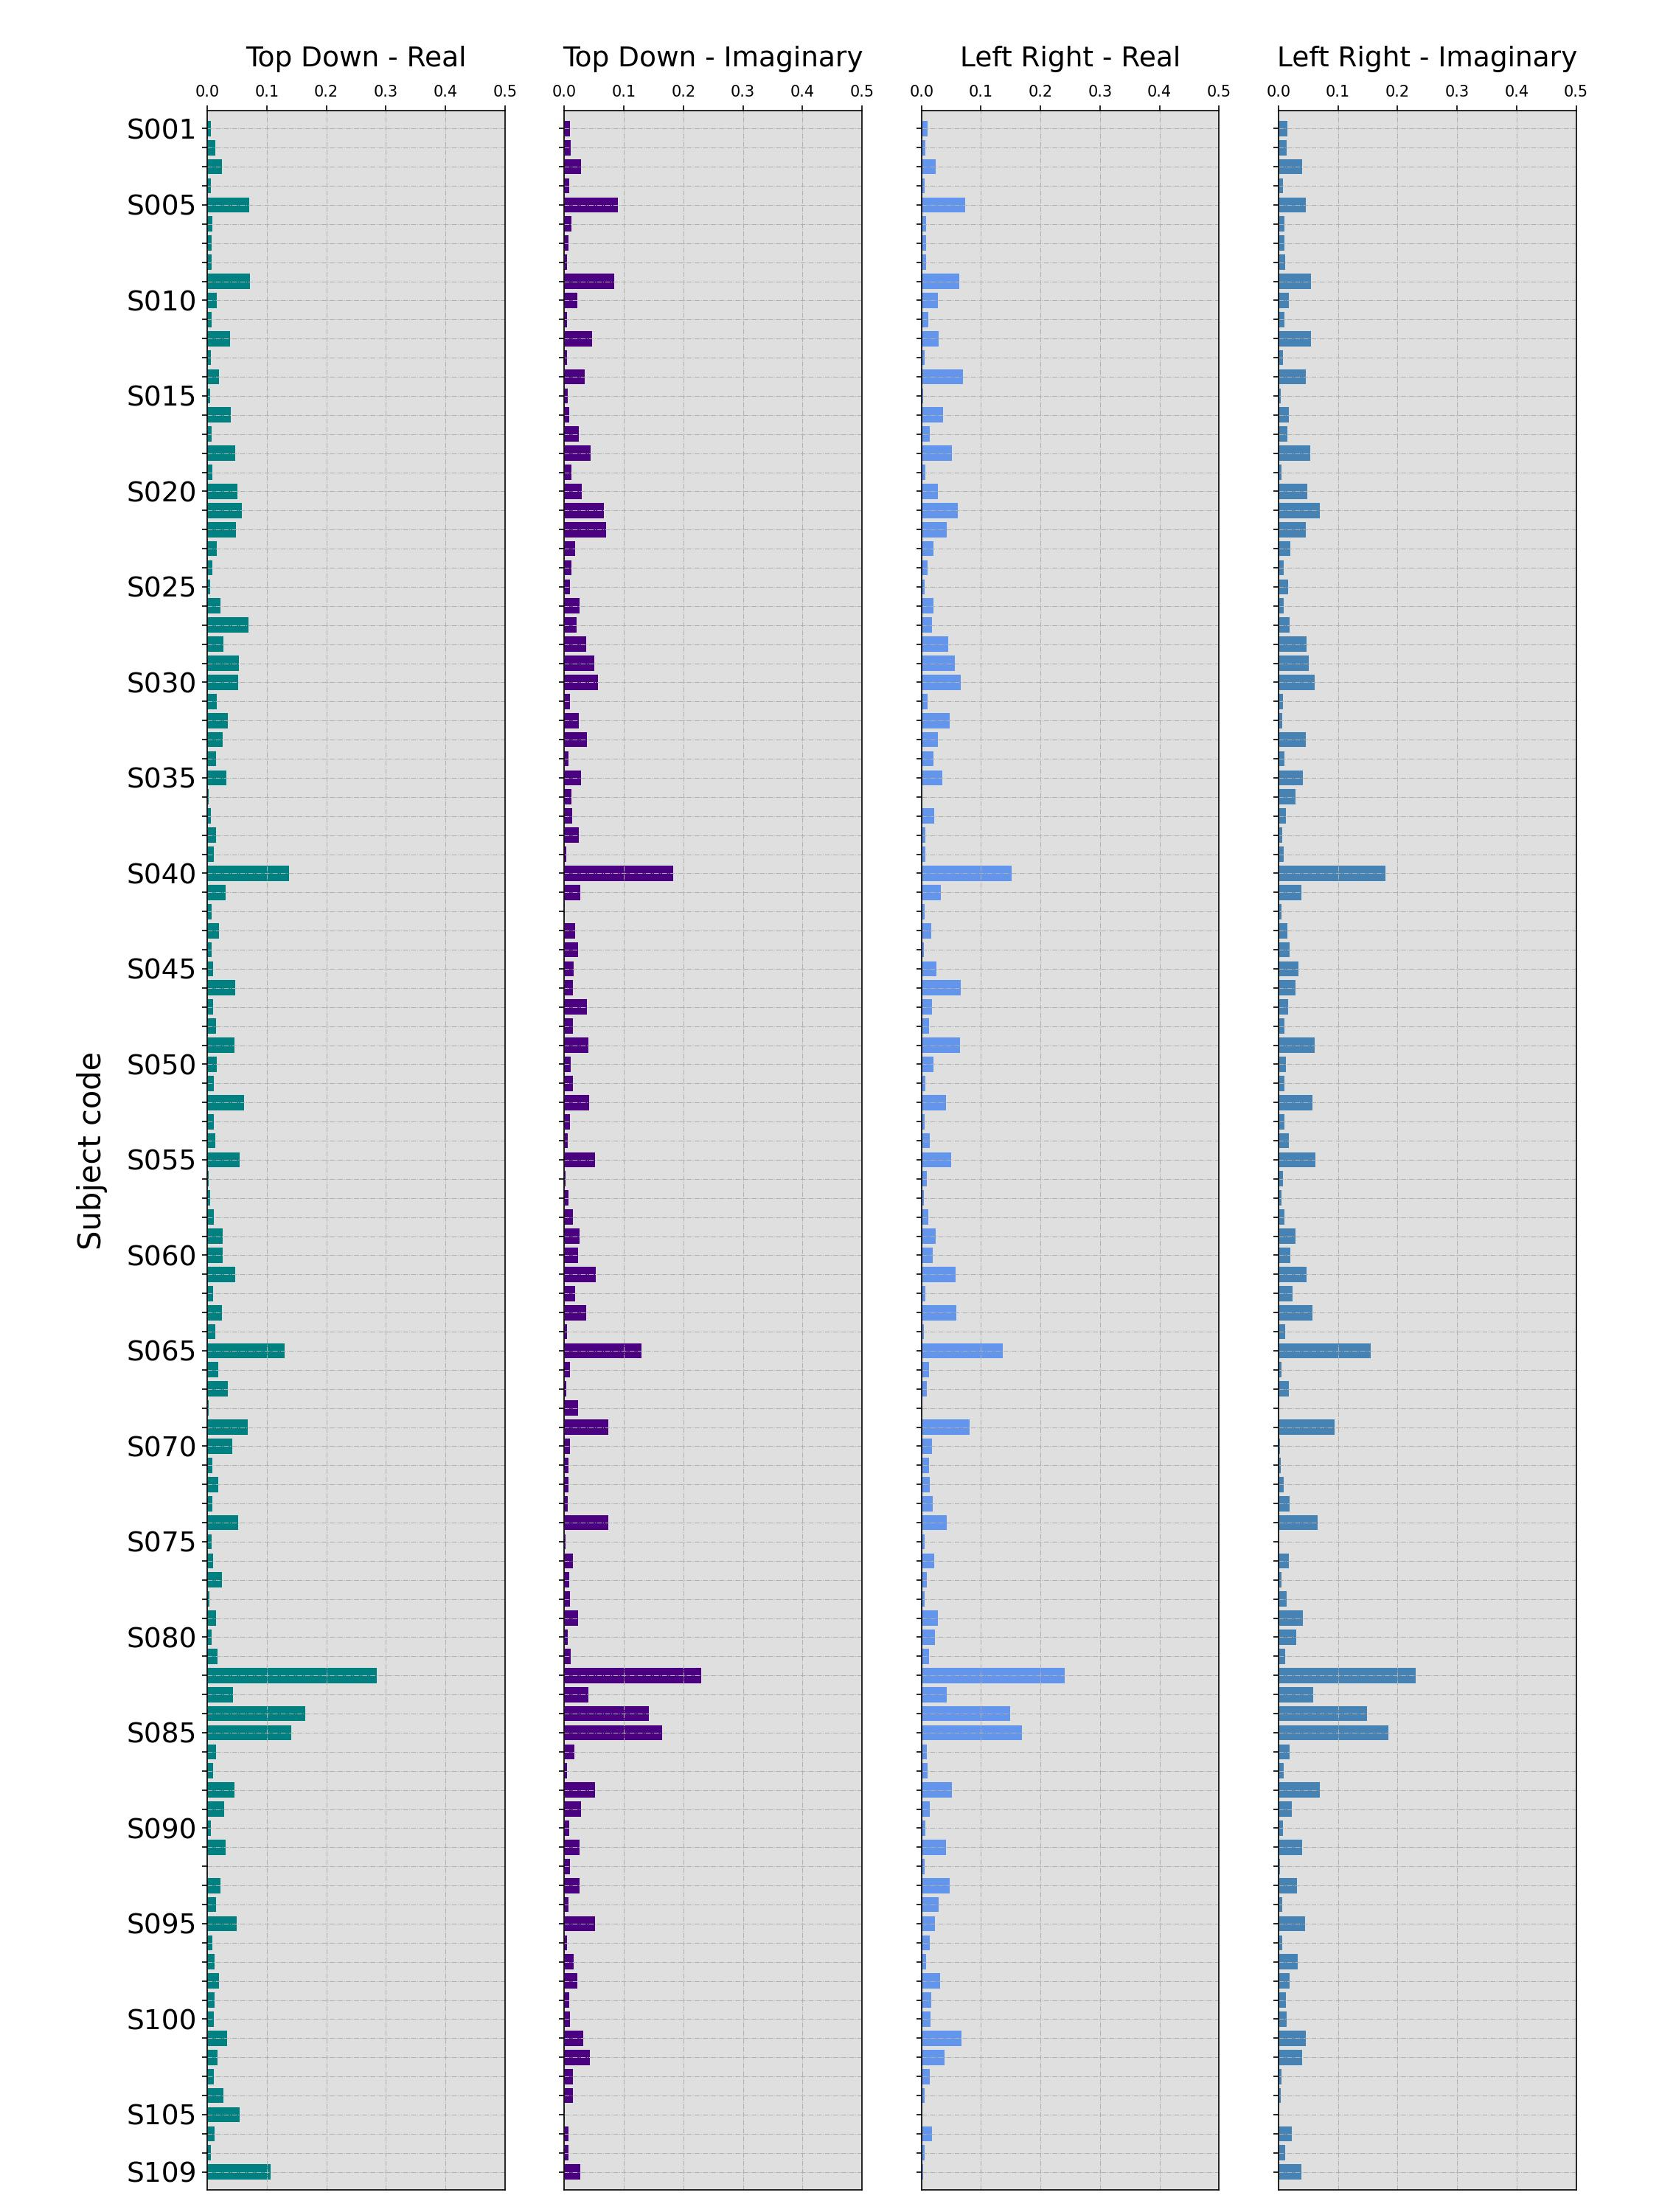
\includegraphics[height=.5\paperheight]{../Figures/art_02/Fig13.jpg}
      \caption{MSE for the Channel $P_{6}$.}
      \label{fig24}
    \end{minipage}
    %%%%%%%

  \end{figure}
  %%%%%%%%%%%%%%%%%%%%%%%%
\end{frame}


\subsection{Algoritmo - biblioteca Python/Zig}

\begin{frame}
  \frametitle{Algoritmo - biblioteca Python/Zig}
  \begin{center}
    pip install zebende \\
    \url{https://pypi.org/project/zebende/}
  \end{center}

\end{frame}


\begin{frame}
  \frametitle{Algoritmo - biblioteca Python/Zig}

  %%%%%%%%%%%%%%%%%%%
  \begin{figure}[!h]
    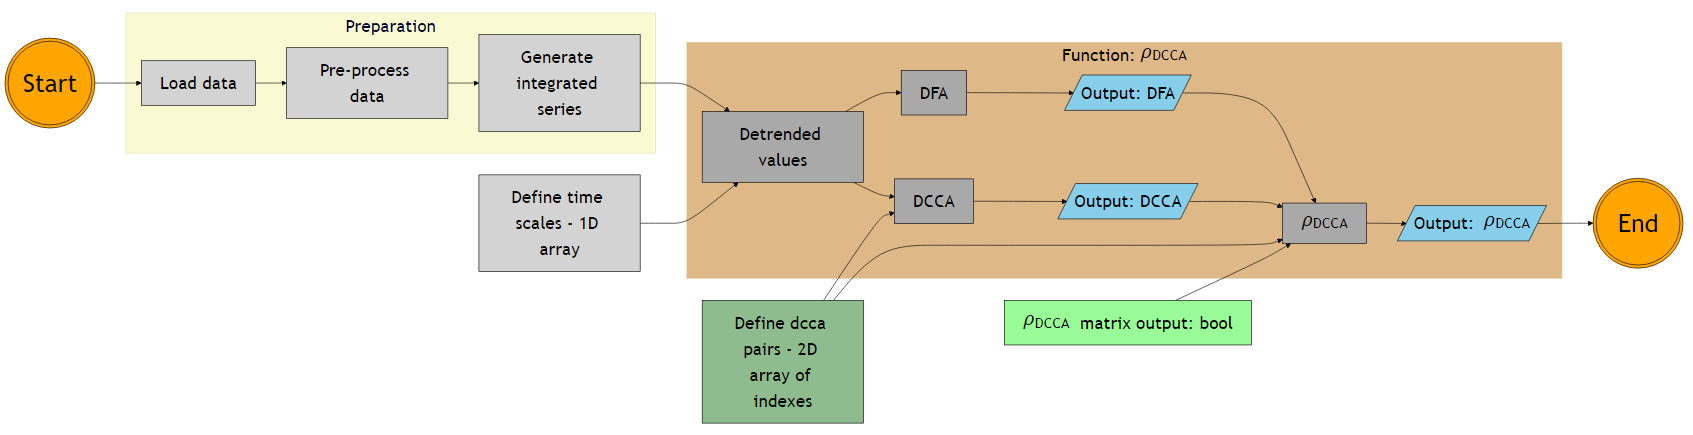
\includegraphics[width=.8\paperwidth]{../Figures/pylib/pdcca_chart.png}
    \caption{\pdcca flowchart.}
    \label{chart_01}
  \end{figure}
  %%%%%%%%%%%%%%%%%%%


\end{frame}

\begin{frame}
  \frametitle{Algoritmo - biblioteca Python/Zig}

  %%%%%%%%%%%%%%%%%%%
  \begin{figure}[!h]
    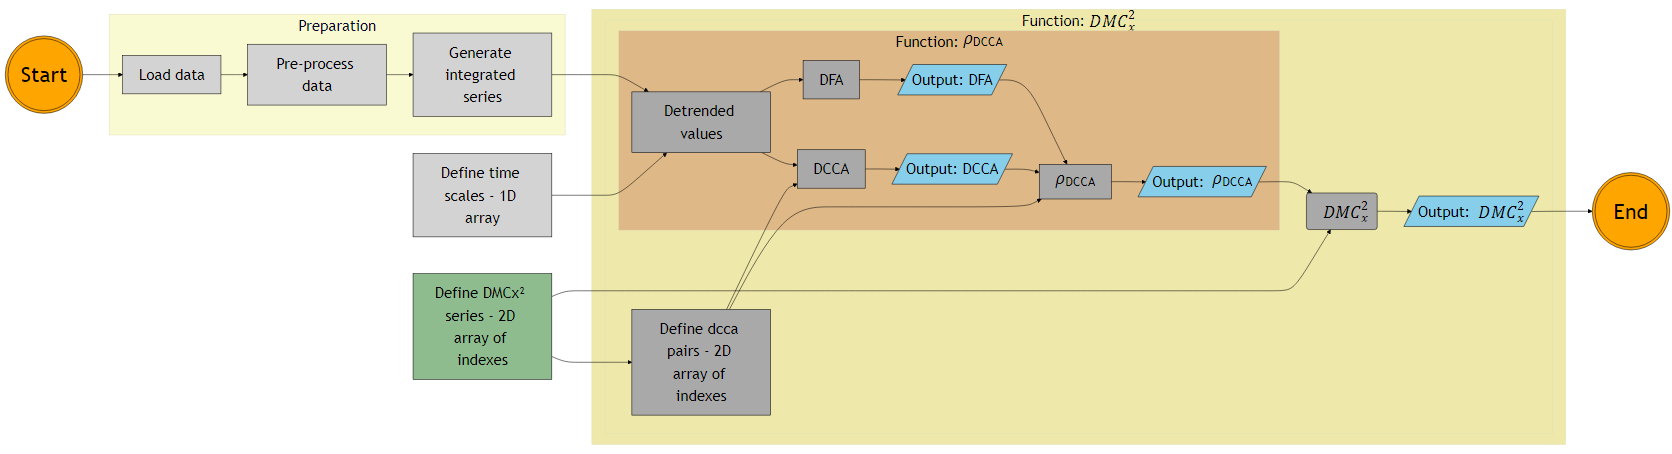
\includegraphics[width=.8\paperwidth]{../Figures/pylib/dmc_chart.png}
    \caption{\dmc flowchart.}
    \label{chart_02}
  \end{figure}
  %%%%%%%%%%%%%%%%%%%


\end{frame}

\begin{frame}
  \frametitle{Otimização}

  Proposta por \citeonline{hartmannRealtimeFractalSignal2013} para o \dfa, transposta para o \dcca~e \pdcca~por~\citeonline{Kapostza2022}.

  \begin{equation}
  \label{eq:sum_opt_x}
  \forall~1<i\leq(N-n),~\sum_{k=i}^{i + n}T_k = \left(\sum_{j=i-1}^{(i+n)-1}T_j\right)~-~T_{i-1}~+~T_{i + n}
\end{equation}

\begin{equation}
  \label{eq:sum_opt_x2}
  \forall~1<i\leq(N-n),~\sum_{k=i}^{i + n}T_k^2 = \left(\sum_{j=i-1}^{(i+n)-1}T_j^2\right)~-~T_{i-1}^2~+~T_{i + n}^2
\end{equation}
\end{frame}

\begin{frame}
  \frametitle{Otimização}

  \begin{equation}
  \label{eq:sum_opt_y}
  \forall~1<i\leq(N-n),~\sum_{k=i}^{i + n}S_k = \left(\sum_{j=i-1}^{(i+n)-1}S_j\right)~-~S_{i-1}~+~S_{i + n}
\end{equation}

\begin{equation}
  \label{eq:sum_opt_xy}
  \forall~1<i\leq(N-n),~\sum_{k=i}^{i + n} (S_k\times T_k) = \left(\sum_{j=i-1}^{(i+n)-1}(S_j \times T_j)\right)-(S_{i-1} \times T_{i-1})+(S_{i + n} \times T_{i + n})
\end{equation}
\end{frame}

\begin{frame}[allowframebreaks]
  \frametitle{Otimização Detrended Saved}
    \bgroup
 \setbeamertemplate{enumerate item}{4.\alph{enumi}}
  \begin{enumerate}
      \item \textbf{Calculando o \emph{Detrended Value}}: Para cada série $X^{j}$ (incluindo a variável dependente) onde  $1 \ge j \ge m$, sendo $m$ o número de séries temporais; para cada escala temporal, em cada caixa $i$, calcula-se o valor de $DV^{j}_{k,i} = (X^{j}_{k,i}-\widetilde{X^{j}}_{k, i})$ e armazena-se em uma matriz. A matrix tem por dimensões $m, n+1$, onde cada linha corresponde a uma série temporal e as colunas correspondem ao número de pontos em cada caixa.
      \item \textbf{Cálculo da função $f_{DFA}^{2}$ para cada caixa}: Calcula-se o valor do \dfa~:\\[10pt]
          $f_{DFA}^{2}(n, i) = \frac{1}{1+n} \sum_{k=i}^{i + n}(DV^{j1}_{k,i})^{2}$;
      \item \textbf{Cálculo da função $f_{DCCA}^{2}$~em cada caixa}: com a matriz $DV$ devidamente preenchida, para uma das $N - n$ caixas de uma mesma escala temporal a função é calculada para todas as combinações de séries temporais duas à duas por:\\[10pt]
          $f_{DCCA}^{2}(n, i) = \frac{1}{1+n} \sum_{k=i}^{i + n}(DV^{j1}_{k,i}) \times (DV^{j2}_{k,i})$
      \item \textbf{Retomando o algorítimo padrão}: Após o cálculo de todas as caixas, aplica-se o passo 5 do \dfa~e \dcca.
    \end{enumerate}
\egroup
\end{frame}

\begin{frame}
  %%%%%%%%%%%%%%%%%%%
  \begin{figure}[!h]
    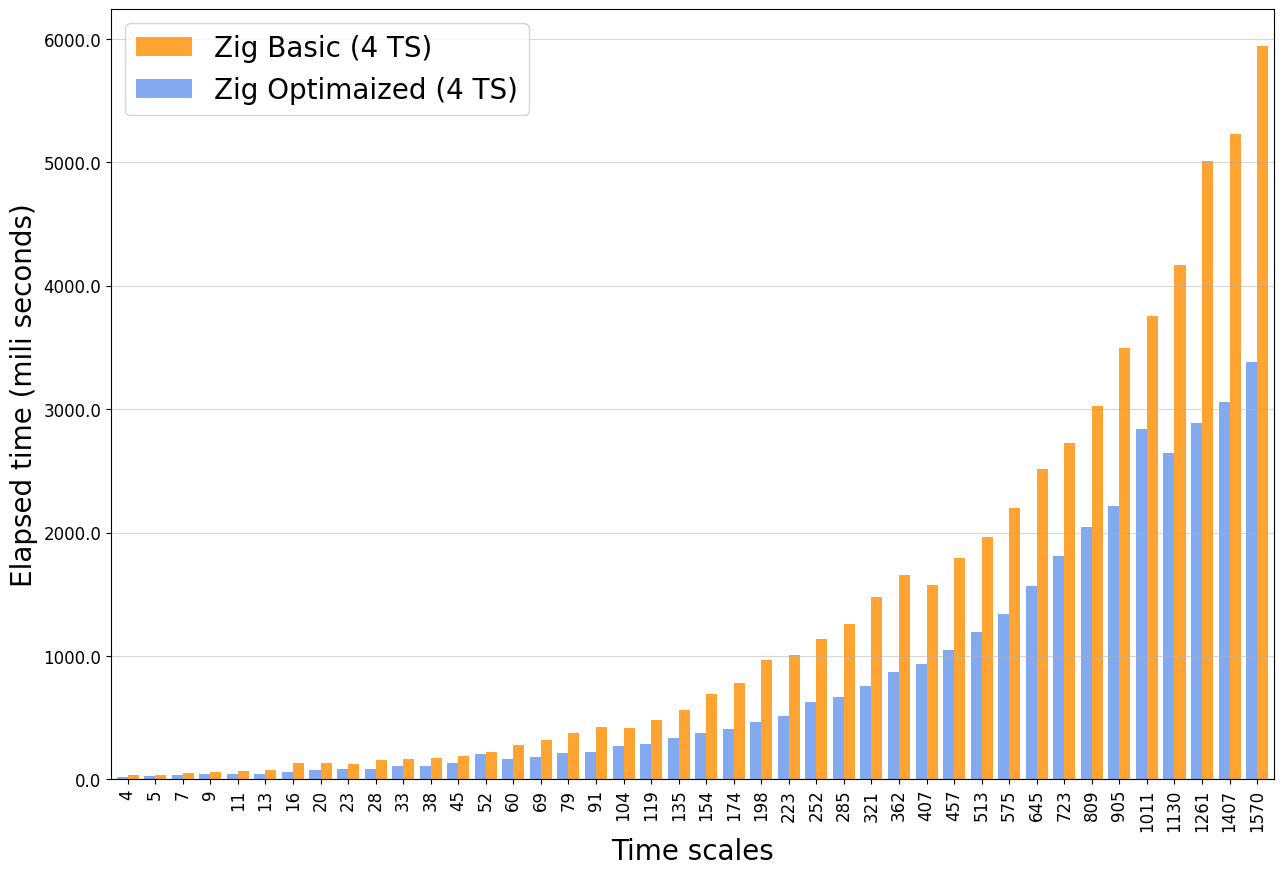
\includegraphics[width=.8\paperwidth]{../Figures/pylib/elapsed_tws_04.png}
    \caption{\pdcca performance with 4 series}
    \label{performance_04}
  \end{figure}
  %%%%%%%%%%%%%%%%%%% 
\end{frame}


\begin{frame}
    \begin{table}[h!]
    \centering
    \caption{Elapsed Time Comparison with four series} \label{tab:time_4}
    \begin{tabular}{@{}l@{\hspace{1.0cm}}l@{\hspace{1.0cm}}l@{\hspace{1.0cm}}l@{}}
      \hline
      Package & Implementation & Elapsed Time(s) & Performance Increase \\
      \hline
      Zebende & Zig (opt) & 35.88  & - \\
      Zebende & Zig (basic) & 59.74 & 66.50\% \\
      DCCA & Python & 447.67 &  1,147.69\% \\
      DCCA & R-Java & 2,206.2 & 6,048.83\% \\
      Zebende & Python & 3,076.23 & 8,473.66\% \\
      DFA & R & 28,116.00 & 78,261.20\% \\
      \hline
    \end{tabular}
  \end{table}
\end{frame}

\begin{frame}
    %%%%%%%%%%%%%%%%%%%
  \begin{figure}[!h]
    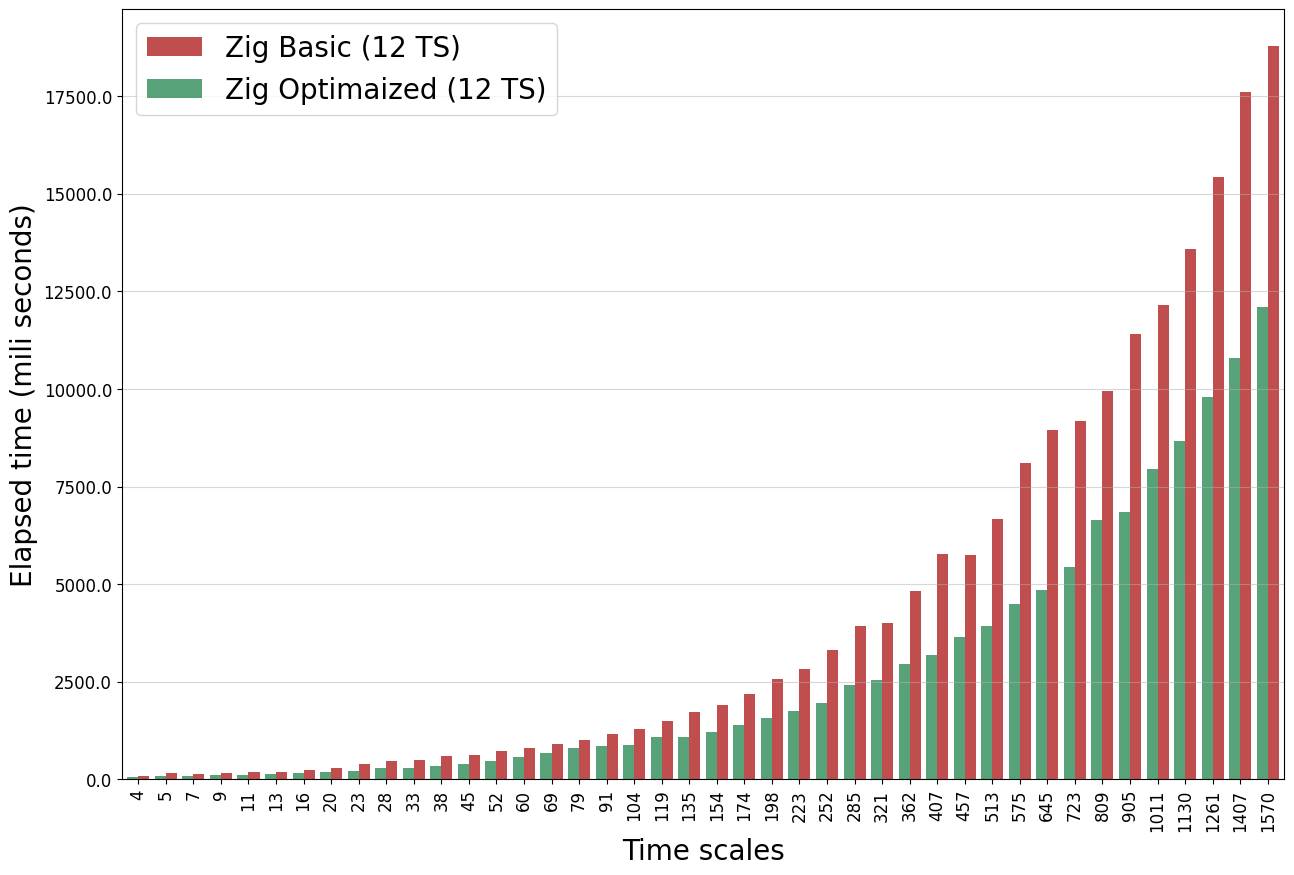
\includegraphics[width=.8\paperwidth]{../Figures/pylib/elapsed_tws_12.png}
    \caption{\pdcca performance with 12 series}
    \label{performance_12}
  \end{figure}
  %%%%%%%%%%%%%%%%%%% 
\end{frame}


\begin{table}[h!]
      
  \centering
  \caption{Elapsed Time Comparison with twelve series} \label{tab:time_12}
  \begin{tabular}{@{}l@{\hspace{1.0cm}}l@{\hspace{1.0cm}}l@{\hspace{1.0cm}}l@{}}
    \hline
    Package & Implementation & Elapsed Time(s) & Performance Increase \\
    \hline
    Zebende & Zig (opt) & 120.55  & - \\
    Zebende & Zig (basic) & 213.08 & 76.64\% \\
    Zebende & Python & 3,761.40 & 3,020.20\% \\
    DCCA & Python & 4,675.17 &  3,778.20\% \\
    DCCA & R-Java & 28,980.00 & 23,939.82\% \\
    DFA & R & 309,276.00 & 256,454.13\% \\
    \hline
  \end{tabular}
\end{table}

\begin{frame}
\frametitle{Maximização do coeficiente \dmc utilizando matriz \pdcca~e $DPDCCA$}
\begin{figure}[!htb]
	\centering
	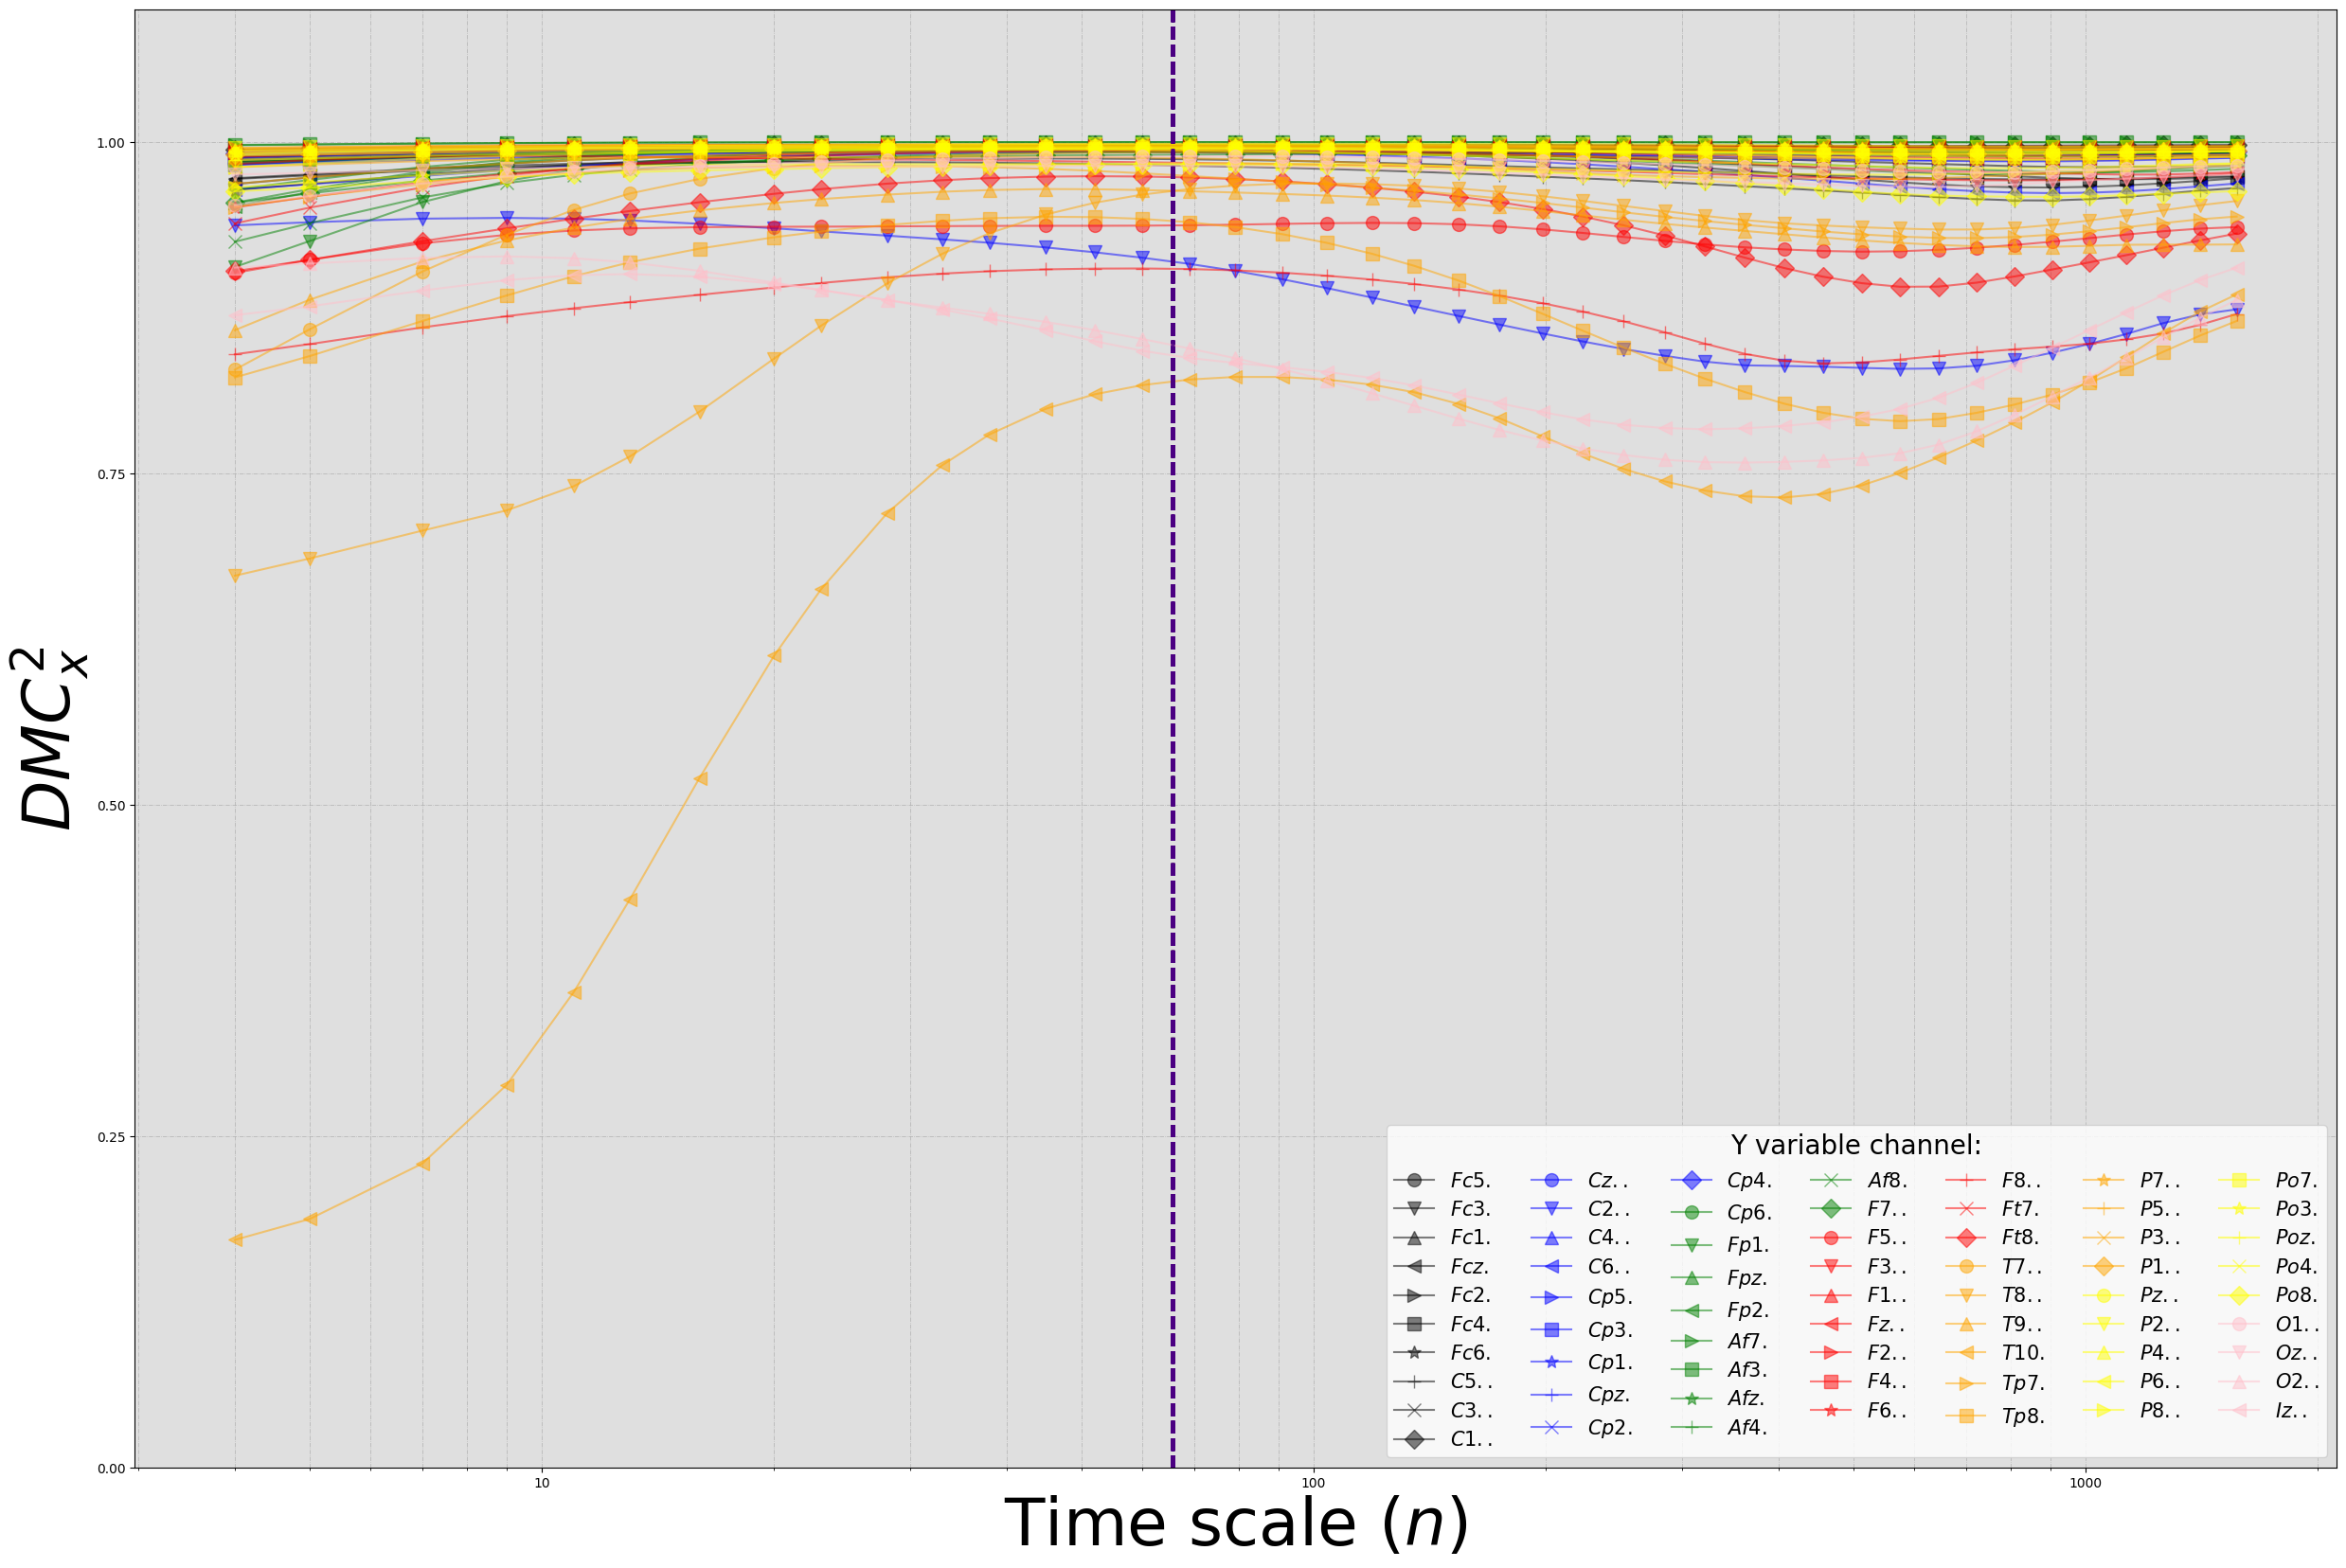
\includegraphics[width=.55\textwidth]{../tese_rev01/Figures/art_03/dmc_all.png}
  % \captionsetup{justification=centering}
  \caption{\dmc~de todo os canais do experimento para cada canal como variável dependente.}

	\label{fig:a03_dmc_total}
\end{figure}
  

\end{frame}

\begin{frame}
\frametitle{Maximização do coeficiente \dmc utilizando matriz \pdcca~e $DPDCCA$}
\begin{table}[h!]
    \centering
    \caption{Maximização do \dmc. $n=4,~ count=8$, referência$= 0.6726$} \label{tab:time_4}
    \begin{tabular}{c|c|c|c}
      \hline
      Critério & canais selecionados & valor & percentual \\
      \hline
      \hline
      \pdcca & T8 Fc6 C6 Cp6 F6 F8 Ft8 P4 P6 & 0.6330  & 94.1108\% \\
      $|$ \pdcca $|$ & T8 Fc6 C6 Cp6 F6 F8 Ft8 P4 P6  & 0.6330 & 94.1108\% \\
      $\Sigma DPDCCA$ & T8 Fc6 C6 Cp6 F2 F4 F6 F8 Ft8 & 0.6329 &  94.0908\% \\
      $DPDCCA$ & T8 C6 Cp6 Fp2 Afz F3 F4 Ft8 P6 & 0.5686 & 84.5341\% \\
      Random & T8 P6 P5 C1 F1 F4 Cp6 Fc1 F6 & 0.3138 & 46.6517\% \\
      
      \hline
    \end{tabular}
  \end{table}
\end{frame}

\frametitle{Variações do \dfa.}



\begin{frame}
\frametitle{Maximização do coeficiente \dmc utilizando matriz \pdcca~e $DPDCCA$}

  \begin{table}[h!]
    \centering
    \caption{Maximização do \dmc. $n=69,~ count=8$, referência$=0.9643 $} \label{tab:time_69}
    \begin{tabular}{c|c|c|c}
      \hline
      Critério & canais selecionados & valor & percentual \\
      \hline
      \hline
      \pdcca & T8 Fc4 Fc6 C4 C6 Cp6 F6 Ft8 Tp8 & 0.9581  & 99.3548\% \\
      $|$ \pdcca $|$ & T8 Fc4 Fc6 C4 C6 Cp6 F6 Ft8 Tp8  & 0.9581 & 99.3548\% \\
      $\Sigma DPDCCA$ & T8 Fc6 C6 Cp6 Ft8 T10 Tp8 P6 P8 & 0.9597 &  99.5189\% \\
      $DPDCCA$ & T8 C6 Cp6 Ft8 T7 T10 Tp7 Tp8 P8 & 0.9572 & 99.2568\% \\
      Random & T8 Fp1 Po7 F7 P6 Cp3 C3 Po4 P2 & 0.8083 & 83.8165\% \\
      \hline
    \end{tabular}
  \end{table}  

\end{frame}


\section{Referências}

\begin{frame}[allowframebreaks]

  \bibliography{../tese_rev01/References/referencias.bib}

\end{frame}

\section*{Obrigado}

\end{document}
